\documentclass[main.tex,fontsize=8pt,paper=a4,paper=portrait,DIV=calc,]{scrartcl}
% Document
\usepackage[T1]{fontenc}
\usepackage[dvipsnames]{xcolor}
\usepackage[nswissgerman,english]{babel}
\renewcommand{\familydefault}{\sfdefault}

% Format
\usepackage[top=5mm,bottom=1mm,left=5mm,right=5mm]{geometry}
%\setlength{\headheight}{\baselineskip}
%\setlength{\headsep}{0mm}

%\usepackage{scrlayer-scrpage}
%\clearpairofpagestyles
%\chead{{\bfseries\TITLE, \AUTHOR, \pagename~\thepage}}

%\addtokomafont{pagehead}{\upshape}

\usepackage{multicol}
\setlength{\columnsep}{2mm}
\setlength{\columnseprule}{0.1pt}

% Math
\usepackage{amsmath}
\usepackage{amssymb}
\usepackage{amsfonts}

% Code
\usepackage{fancyvrb, etoolbox, listings, xcolor}
%\usemintedstyle{bw}

%\newminted[shell]{bash}{
%fontsize=\footnotesize,
%fontfamily=tt,
%breaklines=true,
%frame=single,
%framerule=0.1pt,
%framesep=2mm,
%tabsize=2
%}
%\newminted{css}{
%breaklines=true,
%tabsize=4,
%autogobble=true,
%escapeinside=||,
%stripall=true,
%stripnl=true,
%}

    \definecolor{lightgray}{rgb}{0.95, 0.95, 0.95}
    \definecolor{darkgray}{rgb}{0.4, 0.4, 0.4}
    \definecolor{purple}{rgb}{0.65, 0.12, 0.82}
    \definecolor{ocherCode}{rgb}{1, 0.5, 0} % #FF7F00 -> rgb(239, 169, 0)
    \definecolor{blueCode}{rgb}{0, 0, 0.93} % #0000EE -> rgb(0, 0, 238)
    \definecolor{greenCode}{rgb}{0, 0.6, 0} % #009900 -> rgb(0, 153, 0)
    \definecolor{teal}{rgb}{0.0, 0.5, 0.5}

\lstdefinestyle{code}{
    identifierstyle=\color{black},
    keywordstyle=\color{blue}\bfseries\small,
    ndkeywordstyle=\color{greenCode}\bfseries\small,
    stringstyle=\color{ocherCode}\ttfamily\small,
    commentstyle=\color{teal}\ttfamily\textit\small,
    basicstyle=\ttfamily\small,
    breakatwhitespace=false,         
    breaklines=true,                 
    captionpos=b,                    
    keepspaces=true,                 
    showspaces=false,                
    showstringspaces=false,
    showtabs=false,                  
    tabsize=2,
    belowskip=-5pt
}



% Images
\usepackage{graphicx}
\newcommand{\pic}{\includegraphics[scale=0.3]}
\graphicspath{{Screenshots/}{../Screenshots}}
\makeatletter
\def\pictext#1#2{%
    \@ifnextchar[{%
    \pictext@iiiii{#1}{#2}%
    }{%
      \pictext@iiiii{#1}{#2}[0.5,0.4,0.3]% Default is 5
    }%
}
\def\pictext@iiiii#1#2[#3,#4,#5]{\begin{minipage}{#3\textwidth}\includegraphics[scale=#4]{#1}\end{minipage}\begin{minipage}{#5\textwidth}#2\end{minipage}}
\def\minipg#1#2{%
    \@ifnextchar[{%
    \minipg@iiii{#1}{#2}%
    }{%
      \minipg@iiii{#1}{#2}[0.3,0.6]% Default is 5
    }%
}
\def\minipg@iiii#1#2[#3,#4]{\vspace{0.8mm}\begin{minipage}{#3\textwidth}#1\end{minipage}\begin{minipage}{#4\textwidth}#2\end{minipage}{\vspace{0.8mm}}}
\makeatother

%\newenvironment{minty}[2]% environment name
%{% begin code
%  \begin{minipage}{#1}
%  \begin{minted}{#2}
%}%
%{% end code
%  \end{minted}
%  \end{minipage}
%  \end{minty}\ignorespacesafterend
%} 

% Smaller Lists
\usepackage{enumitem}
\setlist[itemize,enumerate]{leftmargin=3mm, labelindent=0mm, labelwidth=1mm, labelsep=1mm, nosep}
\setlist[description]{leftmargin=0mm, nosep}
\setlength{\parindent}{0cm}

% Smaller Titles
\usepackage[explicit]{titlesec}

%% Color Boxes
\newcommand{\sectioncolor}[1]{\colorbox{black!60}{\parbox{0.989\linewidth}{\color{white}#1}}}
\newcommand{\subsectioncolor}[1]{\colorbox{black!50}{\parbox{0.989\linewidth}{\color{white}#1}}}
\newcommand{\subsubsectioncolor}[1]{\colorbox{black!40}{\parbox{0.989\linewidth}{\color{white}#1}}}
\newcommand{\paragraphcolor}[1]{\colorbox{black!30}{\parbox{0.989\linewidth}{\color{white}#1}}}
\newcommand{\subparagraphcolor}[1]{\colorbox{black!20}{\parbox{0.989\linewidth}{\color{white}#1}}}

%% Title Format
\titleformat{\section}{\vspace{0.5mm}\bfseries}{}{0mm}{\sectioncolor{\thesection~#1}}[{\vspace{0.5mm}}]
\titleformat{\subsection}{\vspace{0.5mm}\bfseries}{}{0mm}{\subsectioncolor{\thesubsection~#1}}[{\vspace{0.5mm}}]
\titleformat{\subsubsection}{\vspace{0.5mm}\bfseries}{}{0mm}{\subsubsectioncolor{\thesubsubsection~#1}}[{\vspace{0.5mm}}]
\titleformat{\paragraph}{\vspace{0.5mm}\bfseries}{}{0mm}{\paragraphcolor{\theparagraph~#1}}[{\vspace{0.5mm}}]
\titleformat{\subparagraph}{\vspace{0.5mm}\bfseries}{}{0mm}{\subparagraphcolor{\thesubparagraph~#1}}[{\vspace{0.5mm}}]

%% Title Spacing
\titlespacing{\section}{0mm}{0mm}{0mm}
\titlespacing{\subsection}{0mm}{0mm}{0mm}
\titlespacing{\subsubsection}{0mm}{0mm}{0mm}
\titlespacing{\paragraph}{0mm}{0mm}{0mm}
\titlespacing{\subparagraph}{0mm}{0mm}{0mm}

%% format cells
\usepackage[document]{ragged2e}
\usepackage{array, makecell}
\renewcommand{\arraystretch}{2}
\newcommand{\mc}{\makecell[{{m{1\linewidth}}}]}


\begin{document}
\begin{table}[h!]
\section{Terms and Definitions}
\begin{tabular}{|m{0.2\linewidth}|m{0.755\linewidth}|}
\hline
AGI Articifial General Intelligence & This is the hypothetical goal of achieving an AI that can perform general task as good or even better than a human. Aka, the goal is to essentially mimic a human in their general life. \\
\hline
Turing test & This is an idea that if a machine can do X task just like a human, aka indistinguishable from the human, then the machine has passed the Turing test. The problem with this however, is that a machine needs to learn to lie, since a human can do this as well -> see the pinoccio problem. The second problem is that certain tasks are too complex for humans but might not be for a machine, in this case the Turing test simply makes no sense. \\
\hline
Machine Learning & Machine Learning is comprised of 3 different techniques. Supervised learning, unsupervised learning and reinforcement learning. Supervised and unsupervised are not that different other tan the presence of the human. Reinforcement learning however is different as the AI is rewarded for "good" behavior/results and "punished" for bad behavior/results. \\
\hline
NLP Natural Language Processing & The research field of trying to achieve both understanding and creation of natural human language by AI. While development has been in the works for quite a while, because AI can't understand context, it is still very much "in beta". \\
\hline
\emph{The 4 Ingredients of Machine-Learning} & 
\vspace{2mm}
\begin{enumerate}
\item Data \newline
In order for a machine to learn anything you need to provide it with data to work with.
\item Cost-Function(Loss) \newline
You need a way to tell your machine what is considered to be good or bad. \newline
Without it the machine can't learn from it's previous endeavors.\newline
\item Model \newline
This can be something simple as 2 parameters like \(y_i = ax_i + b\) or something complicated like a neural network.\newline
We usually use something like \emph{tensorflow} or \emph{pytorch} to define the model\newline
At the end of the day it is always some sort of \textbf{mathematical function!}
\item Optimization
An algorithm that minimizes the amount of parameters needed for the cost function. \newline
Usually something like Stochastic Gradient Descent(SGD), ADAM, RMSProp 
\end{enumerate}
\vspace{2mm}
There are many more, but these 4 are the most important. You might also care about performance optimization\newline
visualization and validation though.\\
\hline
\end{tabular}
\subsection{Representation of words}
\begin{tabular}{|m{0.2\linewidth}|m{0.755\linewidth}|}
\hline
\textbf{\emph{One-hot vector}} & \minipg{ 
This is a vector with 1 value set to 1, this represents the word.\newline
If you now iterate over a sentence, you will end up with a matrix.\newline}
{\pic{2022-09-29_08_51_08.png}}[0.3,0.7]\newline
Problems with this approach\newline
\begin{itemize}
\item high dimensionality\newline
for 100,000 words you would need 100,000 dimensions to the vector.\newline
\item sparse information\newline
The vast majority of the vector aka all but one, is just 0's, this is not data!.\newline
\item no generalization \newline
There is no context for words, no groups, no terms.\newline
For example a car is associated with tires but not with mangos.\newline
This method can't associate anything with anything.\newline
\end{itemize}
\\
\hline
\textbf{\emph{Indexing}} & 
Indexing simply assigns a number to a word. \newline
This approach solves the problem of having a vector with mostly 0's,\newline
but it does not solve the problem of not having context, a mango still has no boundary.\\
\hline
\textbf{\emph{Distributed Representation (dense vectors)}} & \minipg{
This finally solves the issue of context to a certain extend.\newline
We represent a context with a color, if 2 words have the same color in their graph, then there is overlap with these words.\newline
In the following figure the context male is represented in the words man and king, while the context female is represented in the words queen and woman.}
{\pic{2022-09-29_09_14_13.png}}[0.4,0.4]\newline
\minipg{
The way this is done is with a vector that is dense,\newline
this means that this vector has data in multiple dimensions to show context.
}{\pic{2022-09-29_09_19_18.png}}[0.28,0.4]\newline
Important other things to remember:\newline
\begin{itemize}
\item The dot product of 2 vectors becomes 1 if the vectors are parallel.
\item The dot product of 2 vectors becomes 0 if the vectors are orthogonal -> 90 degree angle.
\item The dot product of 2 vectors becomes -1 if the vectors are in the opposite direction.
\end{itemize}\\
\hline
\end{tabular}
\end{table}
\pagebreak
\begin{table}[h!]
\begin{tabular}{|m{0.2\linewidth}|m{0.755\linewidth}|}
\hline
\textbf{\emph{Distance between word vectors}} &
\minipg{
Just like with a regular vector you can calculate the distance between a vector.\newline
Similarly you can also calculate the angle between 2 vectors instead.\newline
}{\pic{2022-09-29_09_34_08.png}}[0.28,0.6]\\
\hline
\textbf{\emph{Finding vector representations}} & 
The obvious question is how do we get the representation of vectors?\newline
\begin{itemize}
\item The first way is to simply use pretrained models that already have the vectors.\newline
\item The other way is to use an embedding layer, this can be done with tools like \textbf{\emph{word2vec}}.\newline
With word2vec you can also use predefined embeddings in order to save you some work.\newline
Another one of these embeddings is \textbf{\emph{GloVe}}.
\end{itemize}
Important tool for creating classes for embedding layers: \textcolor{red}{\textbf{\emph{Keras}}}\\
\hline
\end{tabular}
\subsection{Random Variables}
\begin{tabular}{|m{0.2\linewidth}|m{0.755\linewidth}|}
\hline
\textbf{Discrete and continuous} & \minipg{
Discrete variables are a set of finite numbers.\newline
\large \( X = { 1.5 , 2.678 , 5 , 6.3 , 10 } \)\newline}
{\pic{2022-10-06_08_25_05.png}}[0.3,0.4]\newline
\minipg{
\normalsize Continuous variables are a range of numbers.\newline
\large \( X = (2, 7 ) \) 2 to 7\newline\normalsize}
{\pic{2022-10-06_08_25_08.png}}[0.3,0.4]\\
\hline
Likelyhood and Base information &
The maximum amount of information we can have about a random variable is \textbf{the possible value it can have}, see the set above.\newline
And \textbf{the likelyhood of a specific value appearing}.\\
\hline
\textbf{Notations} & \minipg{
  \emph{\textcolor{teal}{Pr(X=x) is often written in the more compact form P(x) or p(x), or sometimes as PX(x) (there's no formal rule)}}}
{\pic{2022-10-06_08_38_46.png}}[0.3,0.5]\\
\hline
Dice example &
\pic{2022-10-06_08_49_14.png} \pic{2022-10-06_08_49_26.png}\\
\hline
\textbf{Probability Mass Function (PMF)} &
\pic{2022-10-06_08_51_23.png} \pic{2022-10-06_08_52_19.png}\\
\hline
\textbf{Joint Probability} & 
Joint probability is simply the probability of more than 1 thing, in this case 2.\newline
\textcolor{red}{\textbf{If the variables are dependent on each other:}}\newline
\huge \( Pr(A,B) = Pr( A \text{ given } B) * Pr(B) \)\newline
\normalsize \textcolor{teal}{We multiply the chance of A \textbf{(considering A and B can be true at the same time)} with the chance of B.}\newline
For example \(Pr(A \text{ given }B) = 0 \), this means A can't happen when B happens.\newline
\textcolor{red}{\textbf{If the variables are \emph{NOT} dependent on each other:}}\newline
\huge \( Pr(A,B) = Pr(A) * Pr(B) \)\newline
\normalsize \textcolor{teal}{We multiply the chance of A with the chance of B. (independent of each other)}\\
\hline
\textbf{Conditional Probability} & 
This is the \textbf{opposite of Joint Probability with dependence}.\newline
\huge \( P(X,Y) = P(X | Y) P(Y) \)\newline
\normalsize\textcolor{teal}{This is the probability of x and y if y is true. aka probability of x if y is true * probability of y}\\
\hline
\textbf{Bayes Rule} & \minipg{
  Bayes rule uses the fact that we can substitute variables,\newline 
  here we substitute the conditional probability of 2 variables.\newline
  \pic{2022-10-06_09_44_53.png}
}
{\pic{2022-10-06_09_18_12.png}}[0.4,0.4]
\\
\hline
\end{tabular}
\end{table}
\pagebreak
\begin{table}[ht!]
\begin{tabular}{|m{0.2\linewidth}|m{0.755\linewidth}|}
\hline
Confusion Matrix & 
This is simply a matrix that shows correlation of 2 things in a row.\newline
Theoretically, since they are dependent, they should only provide either both true or both false.\newline
However, this is not always the case.\newline
\textcolor{orange}{The general rule: True Positives and True Negatives should always be higher than the other 2!}\newline
\pic{2022-10-20_08_33_25.png}\\
\hline
\end{tabular}
\section{Linear Regression}
\begin{tabular}{|m{0.2\linewidth}|m{0.755\linewidth}|}
\hline
Idea & 
\textcolor{teal}{The basic idea of linear regression is to check for correlation between two sets of data, for example, what is the correlation of mouse size to mouse weight? \newline
Linear regression tries to do this with a simple straight line! It is therefore the easiest way to get a correlation, but it is also not very accurate.\newline
To rectify the bad accuracy, we do this multiple times for a small sets of data, aka for slices of the data.}\\
\hline
Formula and Mean Squared Error & 
\large \(\hat{y}_i = m * x_i + d \)\newline
\( e_i = y_i - \hat{y}_i \)\newline
\huge \( E = \dfrac{1}{2N} \sum_{i=1}^{N}e_{i}^{2} \) \newline
\( MSE = \dfrac{1}{2N} \sum_{i=1}^{N}(y_i - (m * x_i +b))^2 \)\newline 
\normalsize \, \newline
Legend: \newline
\minipg{
\begin{itemize}
  \item \textcolor{orange}{m = \textbf{slope}}
\item \textcolor{orange}{\(x_i\) = x of datapoint}
\item \textcolor{orange}{\(y_i\) = y of datapoint}
\item \textcolor{orange}{\( \delta y_i \) = y of line -> mean(y)}
\item \textcolor{orange}{d = y offset / \textbf{intercept}}
\item \textcolor{orange}{\(e_i\) = single residual -> value of a datapoint}
\item \textcolor{orange}{E = sum of residuals}
\item \textcolor{orange}{N = amount of datapoints}
\vspace{-3mm}
\end{itemize}
}{
  \textcolor{red}{The \( y_i \) inside the MSE is the actual data that we have from our dataset.\newline
  While the \(m * x_i + b\) is the formula that we used. -> linear or polynomial regression.\newline
We are essentially comparing the 2 y's, the one from the data and the one from the calculation.\newline
We then square the difference and do this for every point in the dataset.\newline
Our final calculation will be the \textbf{Mean Squared Error}}
}[0.33,0.4]
\, \newline
\pic{2022-10-27_09_04_09.png}\newline
\textcolor{orange}{You need to first decide what the line is for yourself, this means manual fitting!\newline
Then you can see the Residual Error which would be \textbf{E} in the formula!}\newline
\textcolor{red}{The ultimate goal is to \textbf{MINIMIZE E -> MINIMIZE ERROR!}}\newline
\textcolor{orange}{To do this, we calculate the mean squared error by checking the difference between the data we calculated and our training data.\newline
aka the sum of (training y - calculation y) squared.}
\\
\hline
Least Squares &
\textcolor{orange}{This term simply explains the improvement of fitting a function by calculating them via derivates of slopes:}\newline
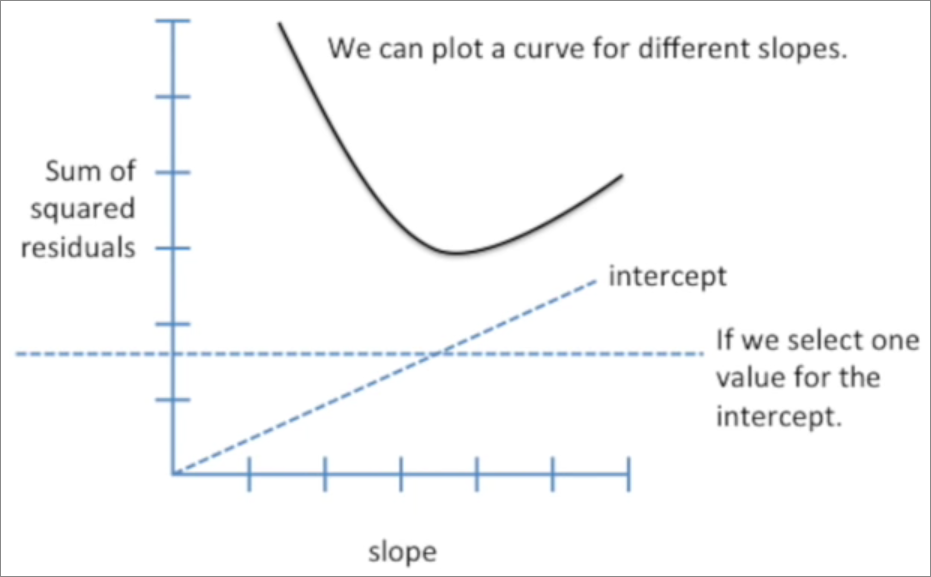
\includegraphics[scale=0.2]{2022-11-10_04_16_23.png}\newline
\textcolor{purple}{As you can see you take the derivate of MSE and slope with respect to slope and try to find a 0 value -> a local minimum or maximum.\newline
And considering we didn't use a fucked up line in the first place, we can be sure that it is indeed a \textbf{local minimum}!}\newline
\minipg{
\textcolor{OliveGreen}{\( \text{derivate in relation to slope} = \dfrac{1}{2N} \sum_{i=1}^{N} \dfrac{d}{dm}(y_i - (m * x_i +b))^2 \)}\newline 
\textcolor{OliveGreen}{\( \text{derivate in relation to slope} = \dfrac{1}{2N} \sum_{i=1}^{N} (2b (bx - y)) \)}\newline 
\textcolor{OliveGreen}{\( \text{derivate in relation to intercept} = \dfrac{1}{2N} \sum_{i=1}^{N} \dfrac{d}{db}(y_i - (m * x_i +b))^2 \)}\newline 
\textcolor{OliveGreen}{\( \text{derivate in relation to intercept} = \dfrac{1}{2N} \sum_{i=1}^{N} 2(x-y+b) \)}
}{
  \textcolor{red}{Now we need to make sure that the derivate is 0! \newline
  \( \text{MSE'} = 0 \)\newline
If this is given, then we have our slope or intercept that will fit best with our current data!}\\
}[0.44,0.31]\\
\hline
\end{tabular}
\end{table}
\pagebreak
\begin{table}[ht!]
\begin{tabular}{|m{0.2\linewidth}|m{0.755\linewidth}|}
\hline
Correlation and Causation &
\textcolor{orange}{Just because something has a mathematical correlation, does not mean that it also has a causality. Some things might be correlated for random reasons, or even simple chance. \newline
For example you might find that the increase in cats is correlated with stormy weather, the data reflects that, but if you know how the weather works, you know that this is utter bs and will never be true.}\\
\hline
Parson Correlation Coefficient & 
\vspace{2mm}
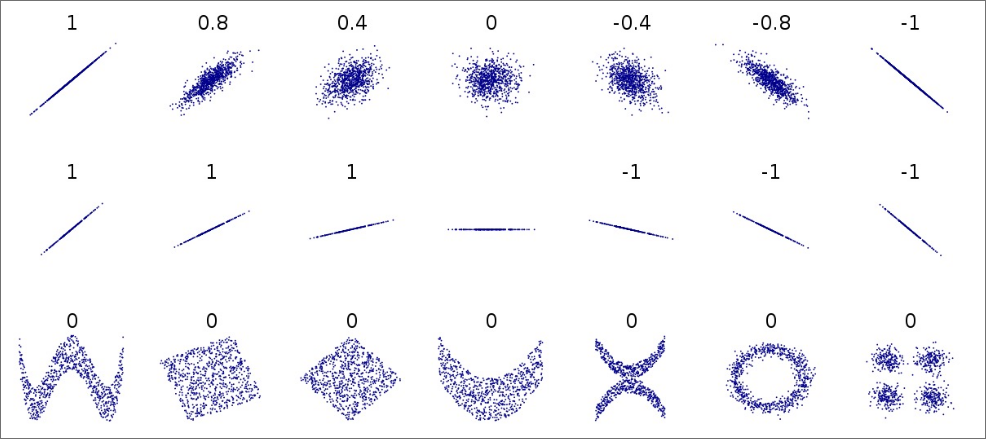
\includegraphics[scale=0.25]{2022-10-27_09_11_27.png}\newline
\begin{itemize}
\item \textcolor{orange}{The correlation is 1 if \textbf{m is positive}, and \textbf{E is 0}.}
\item \textcolor{orange}{The correlation then gradually gets less if there is a deviation between x and y.}
\item \textcolor{orange}{If \textbf{m is negative} and \textbf{E is 0}, then we have -1 correlation. This is still correlation, just negative!}
\item \textcolor{orange}{Should either x or y be constant then calculating the correlation is not possible.}
\item \textcolor{orange}{Lastly, nonsense / nonfunction data, we have correlation 0.}
\vspace{-3mm}
\end{itemize}\\
\hline
Multivariate Linear Regression & 
\textcolor{orange}{This tries to map multiple x data to y -> for example both amount of cats and the amount of dogs correlated to weather, same nonsense, but not 2 times!}\newline
Formula: \( \hat{y}_i = m_{cat} * x_i + m_{dog} * x_i + d \)\newline
\textcolor{teal}{As you can see there is no difference between this formula and the last, other than the fact that we now have two slopes.}\\
\hline
Basic Idea of Gradient Descent & 
\textbf{\textcolor{purple}{You calculate the multivariate linear regression in each step and reduce the error by modifying the parameters in each step}}\newline
\textcolor{orange}{Note that each point represents its own mode, meaning there are different parameters for each point.\newline
This is also how machine learning is done, you might have values like speed and angle that need to be changed in each iteration to take an apex in the perfect manner.}\\
\hline
Gradient Descent & 
\textcolor{orange}{We learned with Least squares that we can take the slope/intercept and see where it is equal to 0 in order to get the best fitting slope or intercept. \newline
However, \textbf{not all function will have a derivate equal to 0 -> min or max}. Also it is quite cumbersome to calculate each slope until we get to 0. It \textbf{might take thousands of steps} until we arrive where we want to be.}\newline
\textcolor{red}{INSTEAD: with gradient descent, we choose a \textbf{Learning Rate}, which will determine our \textbf{step size} in order to skip the part, where we are far away from the optimal 0.\newline
As soon as we approach derivate 0, we take smaller and smaller steps, until we can't improve the value anymore, either we are at 0 now, or 0 is not reachable and we have reached the nearest possible value instead.}\newline
\textcolor{purple}{But where do we take these 2 values from? The \textbf{Learning Rate is a user choice}, while the \textbf{step size is the previous derivate * the learning rate}.}\newline
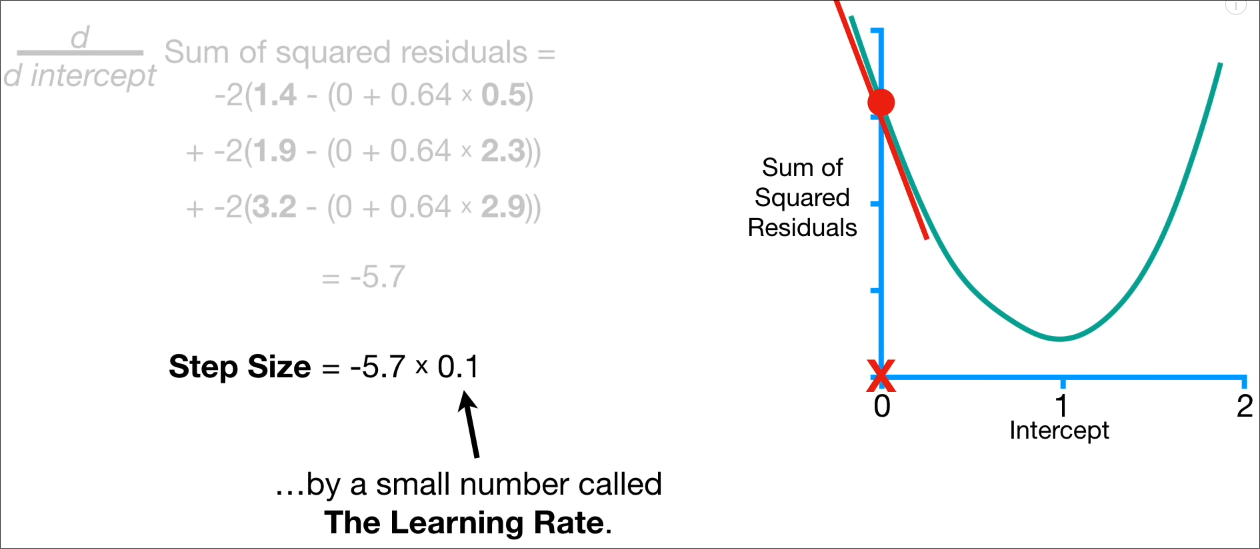
\includegraphics[scale=0.2]{2022-11-10_05_04_33.png}\newline
\textcolor{orange}{Note, the -5.7 is the derivate, therefore we multiply it with the learning rate, which is 0.1 and then we have the next step size.\newline
We can then \textbf{apply the stepsize to the slope or intercept}, whichever we want to calculate.\newline
Then we simply redo this until the derivate will be 0 or close to 0!}\newline
Small notes: Gradient descent usually \textbf{stops when the step size is smaller than the learning rate}\newline
The learning rate is \textbf{usually reduced with each step}.\newline
Also, there is usually a maximum amount of steps that gradient descent will try, for example 1000 steps.\newline
\textcolor{red}{Gradient Descent does \textbf{both intercept and slope at once!} This is also why it is called Gradient descent, because each parameter is a Gradient.}\\
\hline
\textbf{Sochastic Gradient Descent (SGD)} &
The first difference between Gradient Descent and Sochastic Gradient Descent, is that with the second we \textbf{only take random samples of data}.\newline
This allows us to reduce the number of calculations significantly. This is because each iteration of Descent needs the entire MSE to be calculated.\newline
\textbf{Calculating the MSE around random samples of data instead of the full data, decreases calculation time SIGNFICANTLY!}\newline
\textcolor{orange}{2. Difference}\newline
Sochastic Gradient Descent is usually done either with \textbf{just one point per Gradient Descent step}, or with a \textbf{mini-batch -> a small subset of data}, \newline
usually the \textbf{the best way to go is with a mini-batch, as it combines the best of both worlds}.\newline
Also, guess what, another performance increase as you need fewer calculations again!\\
\hline
\end{tabular}
\end{table}
\begin{table}[ht!]
\begin{tabular}{|m{0.2\linewidth}|m{0.755\linewidth}|}
\hline
Annealed SGD & 
\textcolor{black}{The obvious consequence of the \textbf{learning rate} is that \textbf{the learning effect decays over time,}}\textcolor{red}{this is called \textbf{annealing}.}\newline
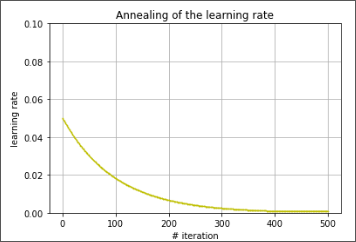
\includegraphics[scale=0.4]{2022-11-04-01_43_27.png}\\
\hline
Limitations & 
\textcolor{purple}{The limitations of this method is that you only use 1 datum -> 1 batch of datapoints for each model. This means that you will have to calculate this over, and over, and over again.\newline
\textbf{In the industry this is usually done in batches of size 32,64,128!}}\newline
\textcolor{orange}{Also, in order to use the SGD the loss function needs to be a \textbf{differentiable function}, this simply means that you can take the derivative of this function at \textbf{every point}. }\newline
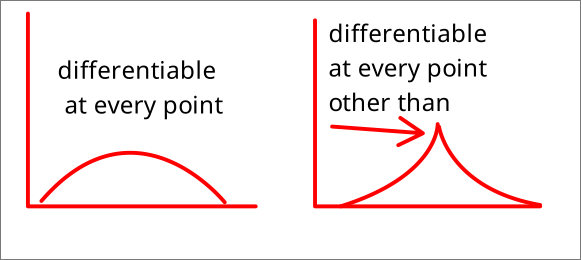
\includegraphics[scale=0.4]{2022-11-04-01_56_28.png}\newline
\textcolor{orange}{On the right side there is the top point where you have 2 interpretations of a derivation, this of course can't be done, so here you would need to define the point manually, or simply use a different function in the first place.}\\
\hline
Generalization Error & 
\textcolor{orange}{This is similar to the correlation but not causation issue. \newline
For example you might have some data that indicates that x is in linear correlation with y, but as soon as you cross a certain threshold, x behaves in an exponential correlation with y.\newline
If you only have the data for the linear part, then you will have a very, very scewed model that \textbf{will not actually represent the real world.}\newline
We call this problem the \textbf{Generalization Error}, where we generalize something without sufficient data.}\\
\hline
Training Error & 
\textcolor{orange}{When you try to fit a model to the data that you have, then you will always have to deal with the problem of potential \textbf{"noisy" data}, it essentially means inaccurate data.\newline
Should you try to perfectly fit a model with this data, then you will likely not achieve a good model as the data is as said not accurate.}\newline
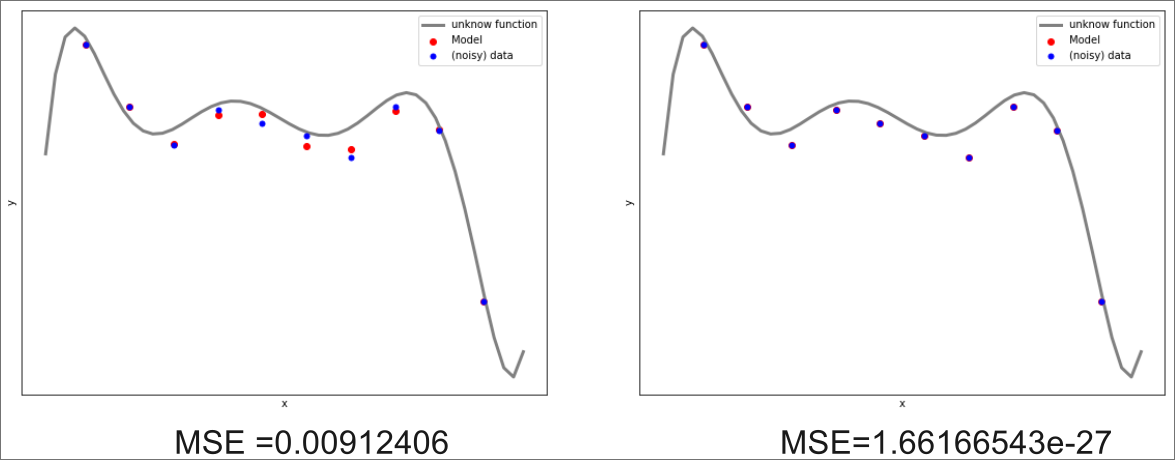
\includegraphics[scale=0.35]{2022-11-10_09_09_47.png}\newline
\textcolor{purple}{As you can see in the image, the left model with less MSE is actually the more accurate model!}\\
\hline
Reducing Generalization Error and Trainign Error with more data & 
\textcolor{orange}{The easiest way is to simply get more data before making a model, this reduces the chance that the samples are error prone, and it also reduces the chance that you will walk into the problem of generalization as you have a lot of data by now.\newline
Problem is that this is not always possible, as data collection can sometimes be very costly, or even impossible.}\\
\hline
Proper Fitting Methodology & 
\textcolor{orange}{Since we have to deal with the generalization error, it is best to \textbf{split the data into 2 sections:}}\newline
\begin{itemize}
\item \textcolor{purple}{80\% of the data for training}
\item \textcolor{purple}{20\% of the data for predictions}
\end{itemize} 
\, \newline
\textcolor{orange}{This means that after we got a model, we can see if it predicts the 20\% of the data. \newline
This way we can limit the generalization error to a certain degree.\newline
\textbf{The data for each split is chosen randomly!}}\\
\hline
Simple models vs Comlex models &
\textcolor{orange}{In comparison to complex models, \textbf{simpler models} have \textbf{a bigger training error} and a \textbf{smaller generalization error}}\newline
Or in a different language, \textbf{smaller models have the chance to underfit}, while the \textbf{complex models have the chance to overfit}\\
\hline
\end{tabular}
\end{table}
\pagebreak
\begin{table}[ht!]
\begin{tabular}{|m{0.2\linewidth}|m{0.755\linewidth}|}
\hline
Bias-Variance & 
\textcolor{orange}{This is the combination that makes up the generalization error, \newline
\textbf{bias indicates a preference towards a certain model}\newline
\textbf{variance indicates the spread of the data}}\newline
\textcolor{purple}{\textbf{A simple model for example has low variance and high bias.}}\newline
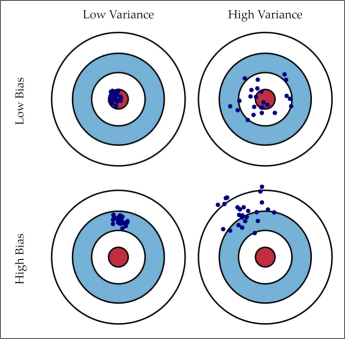
\includegraphics[scale=0.4]{2022-11-10_09_27_19.png}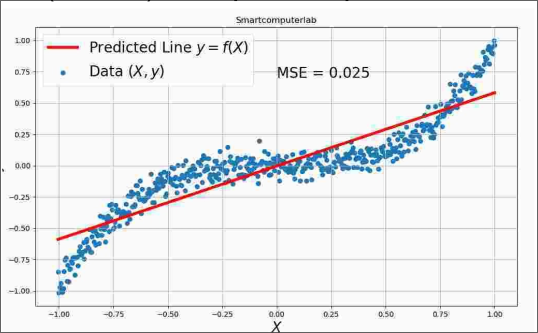
\includegraphics[scale=0.4]{2022-11-10_09_30_46.png}\\
\hline
Goal of Bias and Variance & 
\textcolor{orange}{In the end we want to have the cake and eat it too, aka we want \textbf{low Variance} and \textbf{low Bias}, \newline
the problem is that a complex model gives us low bias, but also gives high variance, while simple models give low variance but high bias.}\\
\hline
Regularization & 
\textcolor{orange}{In order to try to achieve low variance and low bias we introduce another function: \textbf{cost function for training/optimization}\newline
This means we now have 2 functions, the MSE and the optimization function.}\newline
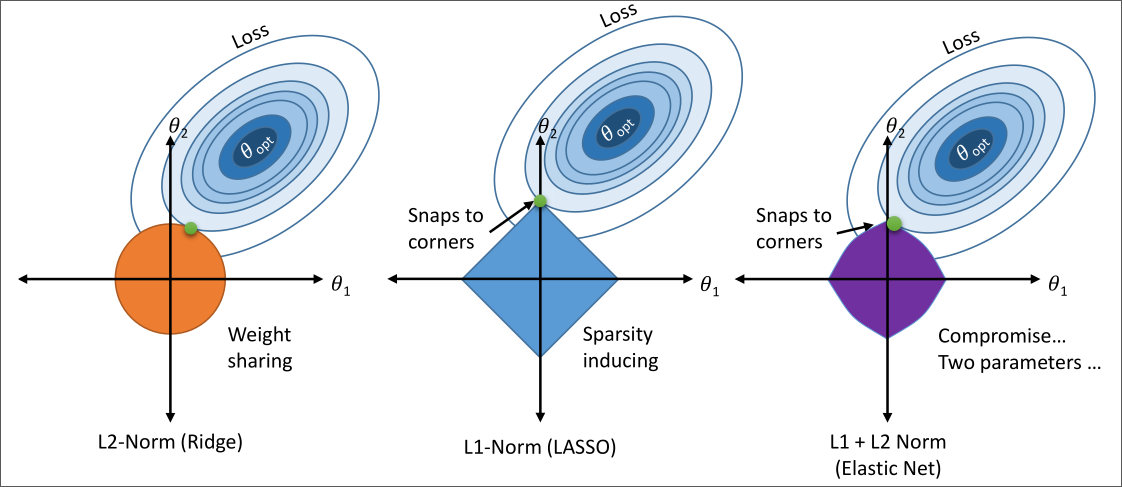
\includegraphics[scale=0.35]{2022-11-10_09_43_03.png}\newline
Regularization tries to introduce a way to \textbf{avoid underfitting or overfitting to the training data}. \newline
This means that we will need to modify our MSE to not do either of these problematic behaviors.\newline
\textbf{Rigde Regularization achieves this by taking the sum of the "corrected paramters by the MSE"}, for example you might have slope and intercept in linear regression, this means that you will have to calculate the \textbf{optimization loss function}, which is the sum of squares of each parameter multiplied by a positive number hat you choose -> \(\lambda\). \newline You then add this function to the base MSE and you have successfully implemted Ridge Regularization:\newline
\, \newline
\textcolor{OliveGreen}{Ridge Regularization:}\newline
\huge \textcolor{red}{\( \text{Ridge MSE} = \dfrac{1}{2N}\sum^{N}_{j=1}(y_j - h(w,x_j))^2 + \lambda \sum^{P}_{i=1} w_i^2 \)}\newline
\normalsize \, \newline 
\, \newline
\textcolor{OliveGreen}{Lasso Regularization:}\newline
\huge \textcolor{red}{\( \text{Lasso MSE} = \dfrac{1}{2N}\sum^{N}_{j=1}(y_j - h(w,x_j))^2 + \lambda \sum^{P}_{i=1} |w_i| \)}\newline
\normalsize \, \newline  
Legend: \newline
\begin{itemize}
\item \textcolor{Orange}{N = sum of datapoints}
\item \textcolor{Orange}{P = sum of parameters}
\item \textcolor{Orange}{w = parameter -> can be multiple ones}
\item \textcolor{Orange}{h = fitting function for example (m * x + d) for linear regression}
\item \textcolor{Orange}{\( \lambda \) = positive number chosen by user 0 to infinity}
\vspace{-3mm}
\end{itemize}\\
\hline
Difference between lasso regularization and ridge regularization & 
\textbf{Lasso regularization can hit the slope 0, while ridge is very unlikely to hit it. This can be seen with the snapping that lasso has!}\newline
\textcolor{red}{Lasso regression can't use gradient descent as it can't be deriviated!!}\\
\hline
\end{tabular}
\end{table}
\pagebreak
\begin{table}[ht!]
\section{Scaling}
\begin{tabular}{|m{0.2\linewidth}|m{0.755\linewidth}|}
\hline
Basic Issue & 
Whenever we have 2 values that should be represented which have different \textbf{weights}, then we need to use scaling in order to make both values have an impact on the graph.\newline
For example if you have one parameter which will affect only a small number, while the other parameter will affect a big number, then changing the second parameter will always \newline
have a bigger impact than changing the first parameter, as it affects a bigger number.\\
\hline
Z-score Normalization &
\textcolor{OliveGreen}{This rescales the dataset to have a \textbf{mean of 0} and a \textbf{standard deviation of 1}}\newline
\textbf{for example: Standardization of a parameter with value 2: \((2-5)/2.138 = -1.4\)}\newline
\, \newline
\huge \( s = \sqrt{\dfrac{1}{N-1}\sum_{i=0}^{N}(X_i - X_{\text{mean}})^2} \)\newline
\, \newline
\( x_{\text{std}} \dfrac{x - X_{\text{mean}}}{s} \)\newline
\normalsize \, \newline
Legend:\newline
\begin{itemize}
\item \textcolor{purple}{Mean: sum of values of data divided by amount of data}\newline
  data points: 2,4,4,4,5,5,7,9\newline
  \(X_{\text{mean}}\) = Mean = 40/8 = 5
\item \textcolor{purple}{s: sample variance}
\item \textcolor{purple}{\(X_{\text{std}}\): sample standard deviation}
\end{itemize} 
There is another issue that feature scaling will fix, \textbf{regularization is biased, meaning it will punish higher value parameters harder!}\newline
This is yet another reason why we want to use scaling in order to reduce the effect that regularization has on our parameters.\\
\hline
\end{tabular}
\section{Model Evaluation}
\begin{tabular}{|m{0.2\linewidth}|m{0.755\linewidth}|}
\hline
2-way Holdout & 
2-way Holdout is the model that we have been using until now with the 20-80 split in data to train and test your model:\newline
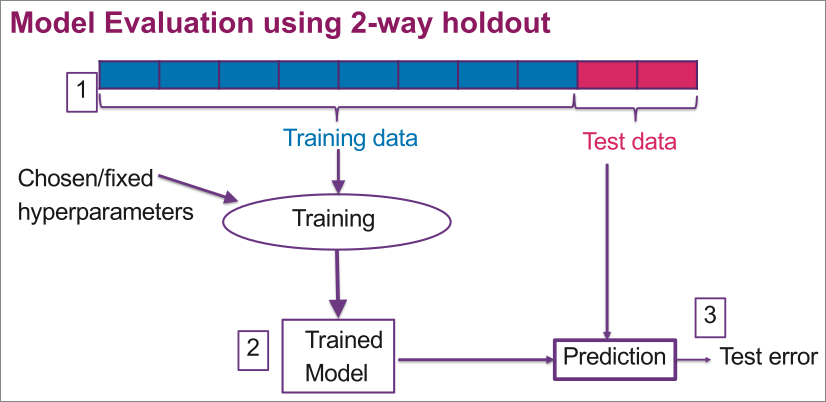
\includegraphics[scale=0.3]{2022-11-17_08_44_33.png}\\
\hline
3-way Holdout & 
\minipg{
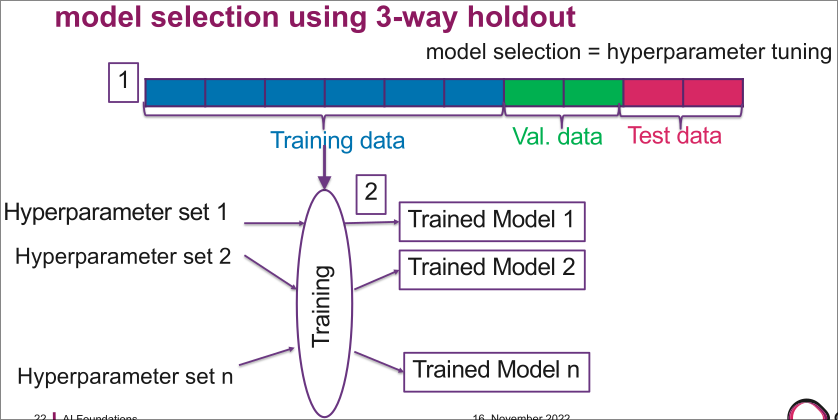
\includegraphics[scale=0.3]{2022-11-17_08_47_18.png}
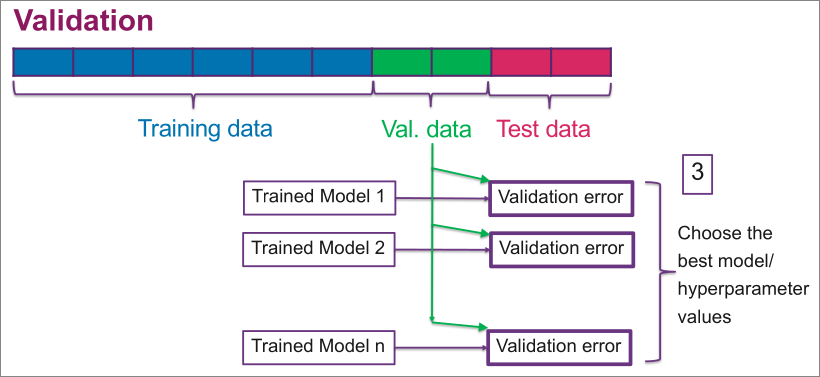
\includegraphics[scale=0.3]{2022-11-17_08_47_22.png}
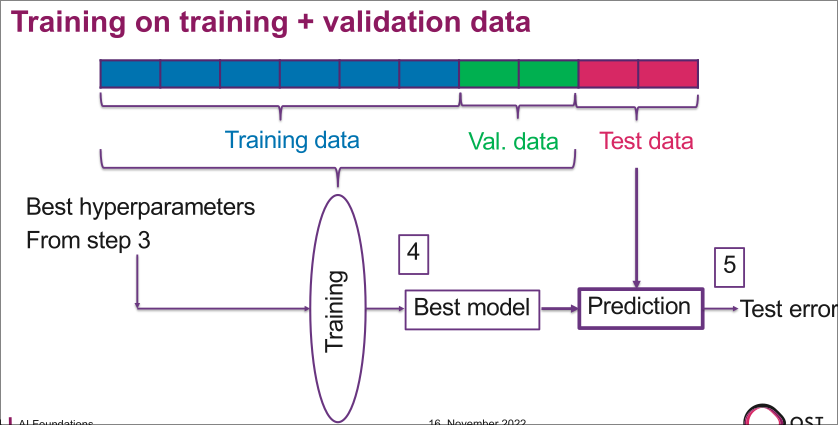
\includegraphics[scale=0.3]{2022-11-17_08_47_31.png}
}{
The idea here is to always have different possibilities of each step, meaning \textbf{multiple parameters to train multiple models}, then \textbf{test each model on the test data}.\newline
Then you \textbf{use the best parameters, meaning the ones that are the closest to both the training data AND the test data.}\newline
At the end you have your test error just like with the 2-way holdout.\\
}[0.45,0.3]
\\
\hline
\end{tabular}
\end{table}
\pagebreak
\begin{table}[ht!]
\begin{tabular}{|m{0.2\linewidth}|m{0.755\linewidth}|}
\hline
Final Model & 
In both 2-way and 3-way holdout, you can have a final model calculation: \newline
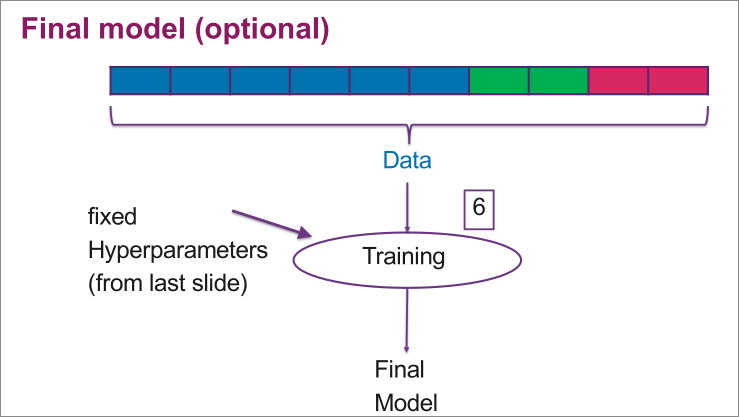
\includegraphics[scale=0.3]{2022-11-17_08_54_03.png}\\
\hline
Problems with Holdout& 
In general, the test data will only be a subset of the entire dataset, and if we get unlucky, the test data might be shit.\newline
In other words, \textbf{it might have extremes or it might have too many values that are just right for our predicted line, but not for the actual line...}\newline
The solution would be splitting the data further, but how? Find out below kekw\\
\hline
k-fold Cross Validation & 
\textbf{k-fold Cross Validation is just one variant of cross validation, you can theoretically implement your own, but this one if the most used.}\newline
\textcolor{OliveGreen}{In k-fold cross validation, we split the data multiple times until we have had each split as validation data once, while the rest servers as the training data during that time:}\newline
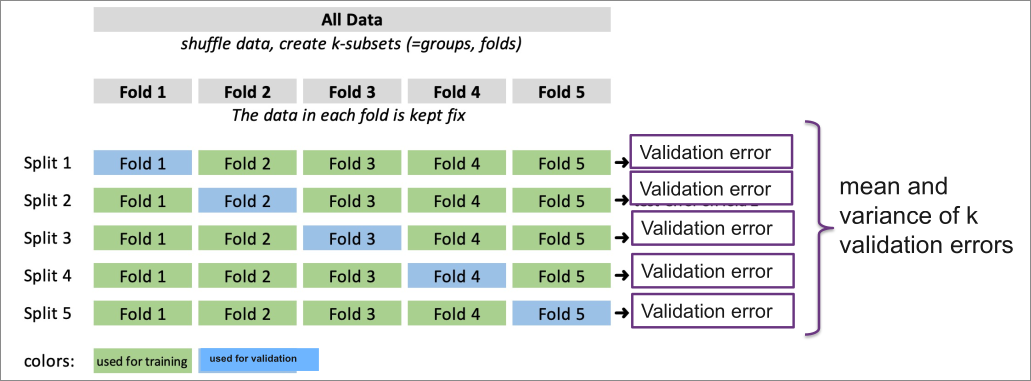
\includegraphics[scale=0.3]{2022-11-17_09_07_59.png}\newline
At the end you can calculate the \textbf{mean and variance of k validation errors}. \textbf{This mean will now be your Validation Error!}\newline
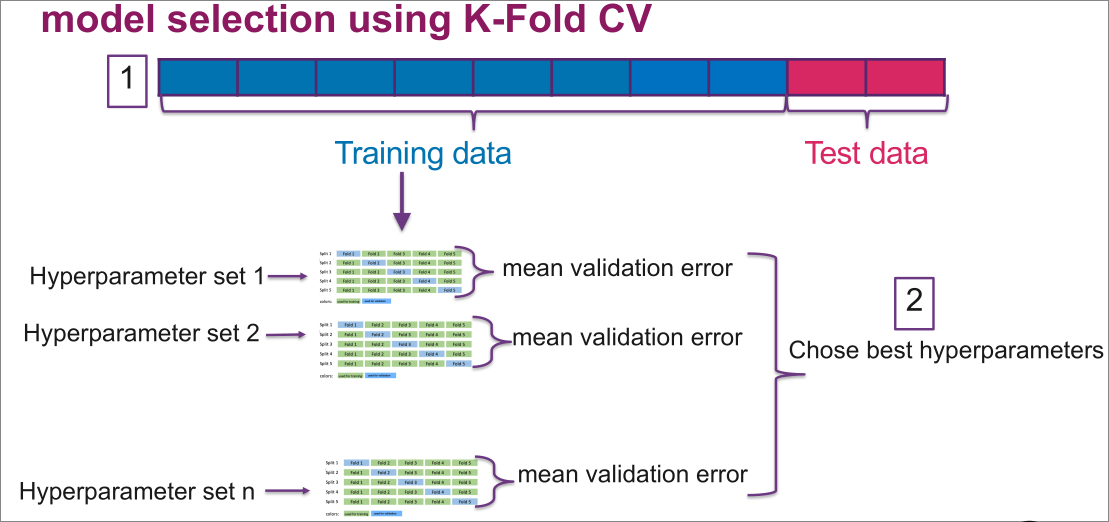
\includegraphics[scale=0.3]{2022-11-17_09_12_34.png}\newline
\textcolor{red}{Note, \textbf{the test data is not included in the fold, it is NOT touched until you want to test your models.}}\\
\hline
Binary Probability & 
In many cases we want to know a yes or no answer, based on a prediction, for example is group A applicable for this study  based on their height. You can't just measure everyon so you have to take predictions based on the groups other specifications, eg. you might know their age range, sex, etc. From this data you can get a predicition for the height, which then leads you to your answer, but, this answer is not binary, so what do we do? \newline
\textcolor{OliveGreen}{Simple, we use a treshold on where we simply say that there we will consider the answer as yes, and everything below is a no.}\newline
\minipg{
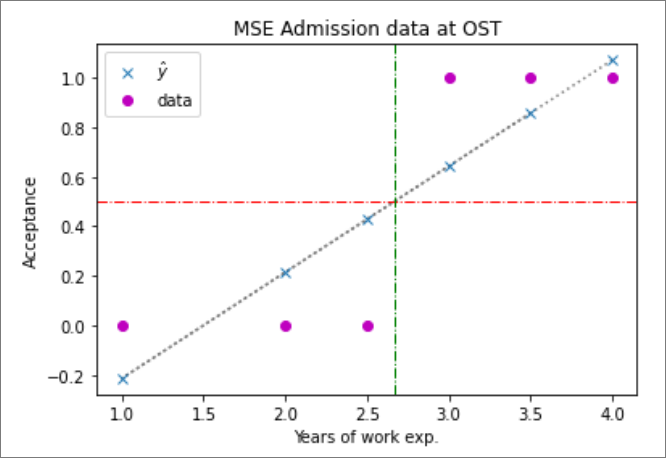
\includegraphics[scale=0.4]{2022-11-24_08_45_49.png}
}{
  There is however a problem with this, you can't use this in combination with linear regression, as we only have either 0 -> false, or 1 -> true. \newline
  However, we can use what is called \textbf{Logistic Regression}, this will work on the probability instead of the outcome data, which again in our case is 0 or 1 because of our threshold!
}[0.48,0.28]\\
\hline
\end{tabular}
\end{table}
\pagebreak
\begin{table}[ht!]
\begin{tabular}{|m{0.2\linewidth}|m{0.755\linewidth}|}
\hline
Logistic Regression & 
As already described before, we now need something that will work on the probability to regress on, how about the signum function, which would turn pretty much any number to 1 or 0?\newline
\minipg{
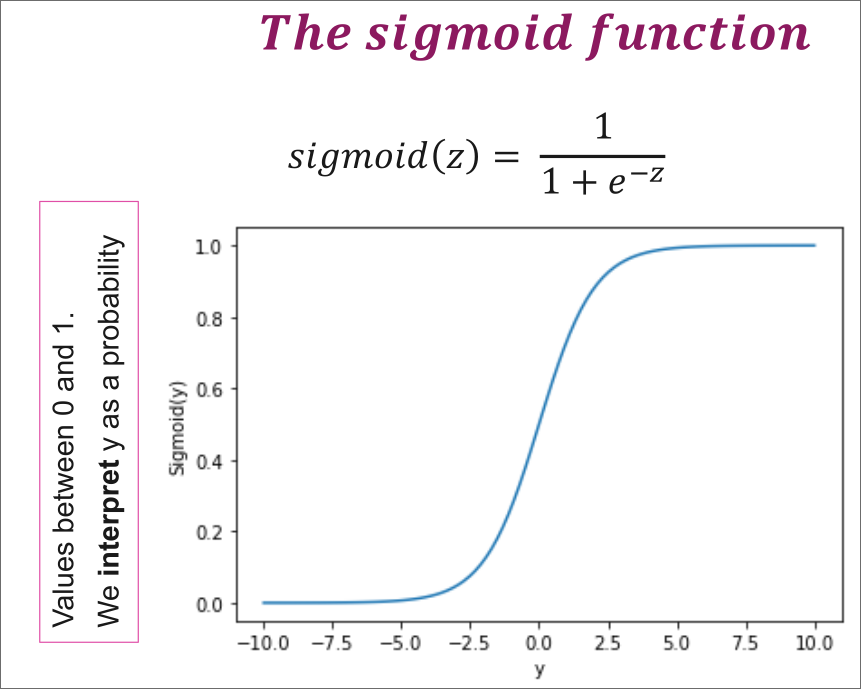
\includegraphics[scale=0.25]{2022-11-24_09_04_16.png}\newline
}{
  \large \textcolor{purple}{\( sigmoid(z) = \dfrac{1}{1 + e^{-z}}\)}\newline
  \large \textcolor{purple}{\( z = h(w,x) = w_1x_1 + w_2x_2 + \text{...} + w_nx_n \)}\newline
  \normalsize \textbf{The x represents the data that we have, while w is the value to figure out -> unknown line}
}[0.46,0.3]
\\
\hline
Log(odds) & 
Because of the division on odds, \textbf{the values that indicate odds in favor of the quotient have a higher magnitude}, in other words, \textbf{should the odds not be in "our" favor, then the number will be between 0 and 1}, however, \textbf{should the odds be in "our" favor, then the number will be between 1 and infinity!!}\newline
In order to solve this issue, we can take the log of the odds with base e.\newline
This will make the calculation perfectly symetrical again, with both sides of the odds being represented properly.\newline
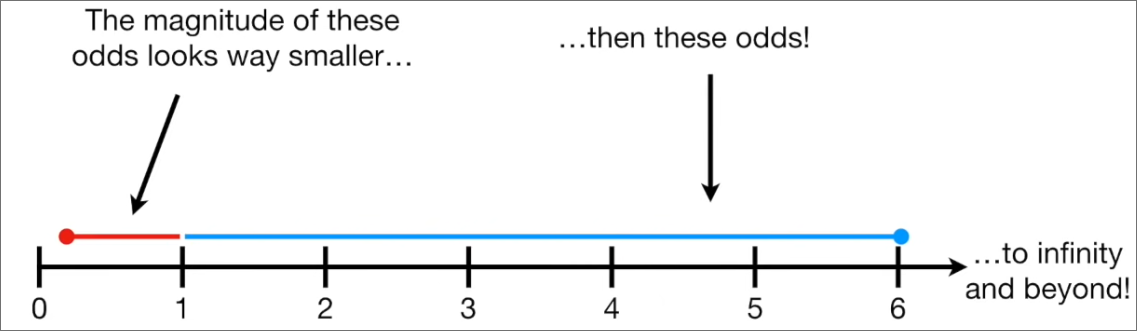
\includegraphics[scale=0.25]{2022-11-24_12_32_32.png} 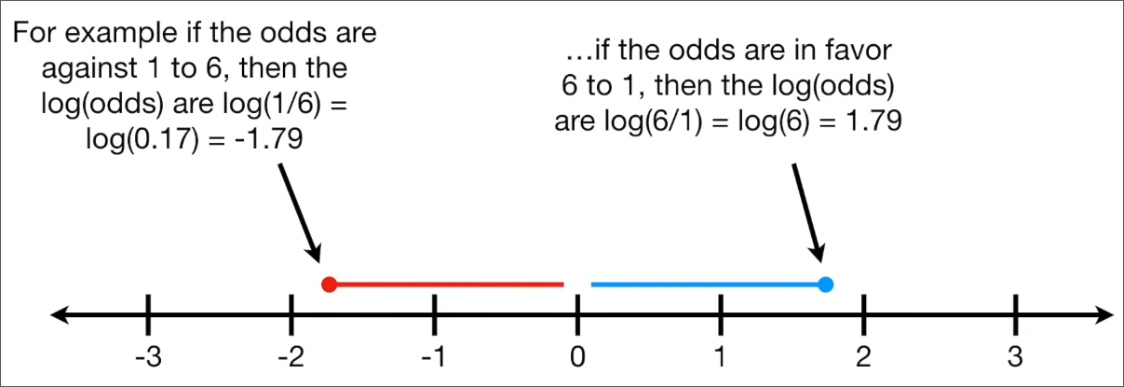
\includegraphics[scale=0.25]{2022-11-24_12_32_39.png}
\\
\hline
Odds vs Probability & 
The difference in odds is that it only considers a possiblity with the opposite of that, while probability considers the possiblity of something against EVERYTHING.\newline
Eg. \textbf{my team winning vs not winning -> odds, my team winning vs my team winning, tied, and losing -> probability}\newline
\textcolor{red}{Odds can however also be displayed by using probabilities instead of numbers, aka the probability of winning divided by the probability of losing is still odds!}\newline
Consider the ratio of winning as 5, tied as 3 and losing as 4.\newline
Probability for winning: \( \dfrac{5}{5+3+4} \) \newline
Odds for winning: \( \dfrac{5}{4} \) OR \textcolor{red}{with probabilities:\( \dfrac{\dfrac{5}{8}}{\dfrac{4}{8}} \)}\newline
Note, the second is called \textbf{logit function} and can be shortened to this: \textcolor{RubineRed}{\( odds = \dfrac{p}{1 - p} \)}\newline
\\
\hline
Odds Ratio &
While the previous examples were also ratios, we mean something different with this, namely the division of 2 odd calculations.\newline
This comes into play when you want to check correlation between two traits based on data.\newline
Let's take the following idea, we have mice some of which are obese, and some have heart issues.\newline
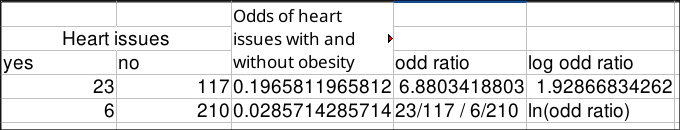
\includegraphics[scale=0.4]{2022-11-24_12_59_20.png} \newline
As you can see the odd ratio is the odds of obese mice having heart issues to the odds of non obese mice having heart issues.\newline
Then we take the log just like regular odds, in order to make the result symetrical!\\
\hline
\end{tabular}
\end{table}
\pagebreak
\begin{table}[ht!]
\begin{tabular}{|m{0.2\linewidth}|m{0.755\linewidth}|}
\hline
Statistically Significant Odds & 
For logistic regression we use the \textbf{Wald test} to check whether or not our odds ratio is statistically significant.\newline
What we do is calculate the \textbf{standard deviation},  this is how most values of the \textbf{odds ratio} will be spread away from 0.\newline
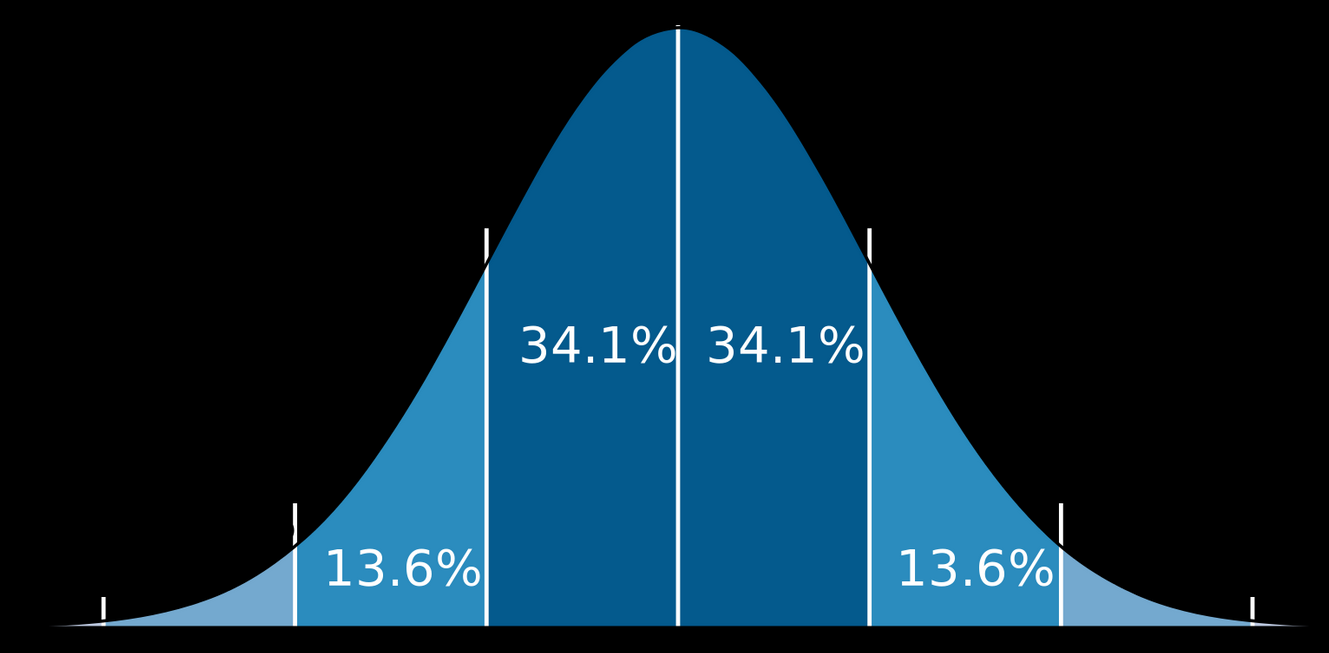
\includegraphics[scale=0.2]{2022-11-24_01_18_37.png}\newline
here the standard deviation if the 34.1\% mark.\newline
However instead of calculating every odds ratio, we can caluclate the following instead to get the same value:\newline
\large standard deviation = \( \sqrt{\dfrac{1}{23} + \dfrac{1}{6} + \dfrac{1}{117} + \dfrac{1}{210}} \)\newline
\normalsize As you can see these are the values from the mice obesety to heart problems chart.\newline 
\textcolor{red}{Should this value be either \textbf{smaller than -2 or bigger than 2, then it is statistically significant!}}
\\
\hline
&
The odds ratio is the division between the probability of data being 1 and data being 0.\newline
\large \textcolor{purple}{\( odds(p) = \dfrac{p}{1-p} \)}\newline
\large \textcolor{purple}{\( log ( \dfrac{Pr(y=1|x)}{1-Pr(y=1|z)} = e^{W^{T}x} ) \)}\newline
Estimated Probility:\newline
\large \textcolor{purple}{\( Pr(y=1|x;W) = \dfrac{e^{W^T x}}{1+e^{W^T x}} = \dfrac{1}{1 + e^{W^T x}} = p(x) \)}\newline
\normalsize \, \newline
Note: \( W^T x \) is the same as \( w_ix_i \) in matrix form, in other words, the T stands for \textbf{Transform}.\newline
\large Loss Function:\newline
\textcolor{purple}{Minimize Cost(W) =\( \dfrac{-1}{N}\sum^{N}_{i=1}(y_i * log(p(x_i)) + (1-y_i)) * log(1 - p(x_i)) \) }\newline 
\normalsize \, \newline
For the loss function, we learned that we want to penalize every value that is wrong, eg here too large or too low.\newline
Here we have the 2 log on prediction for it to be true and for it to be false:\newline 
\begin{itemize}
\item \textcolor{purple}{w = parameter}
\item \textcolor{purple}{p(x) = probability of something with value x}
\vspace{-3mm}
\end{itemize}
\, \newline
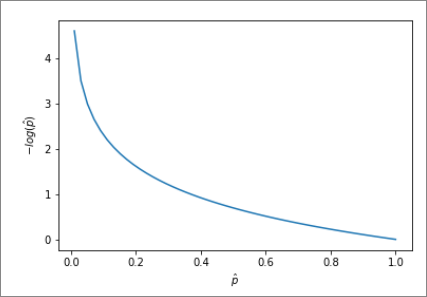
\includegraphics[scale=0.4]{2022-11-24_09_26_52.png} 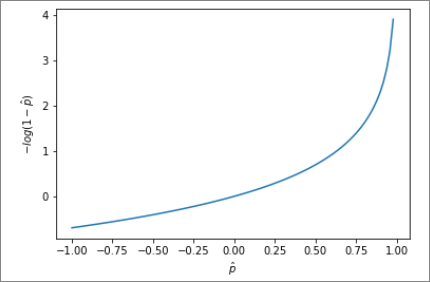
\includegraphics[scale=0.4]{2022-11-24_09_26_55.png}\newline
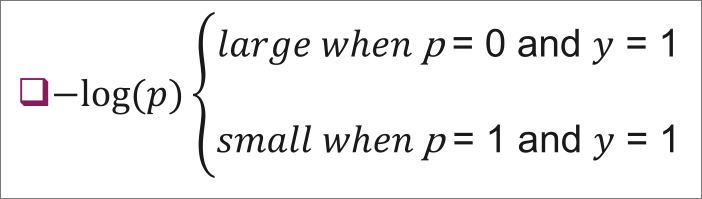
\includegraphics[scale=0.25]{2022-11-24_09_30_09.png} 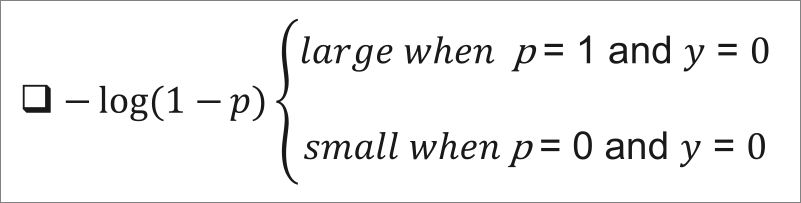
\includegraphics[scale=0.25]{2022-11-24_09_30_11.png}\newline
\textcolor{red}{Here we need to make sure that our coeffiecients/parameters get p to 0 when y is 0 and p to 1 if y is 1.}\newline
\\
\hline
Confusion Matrix with Logistic Regression & 
We already talked about True/False Positives/Negatives, this now fits well into our system of evaluating things that can either be true or false.\newline
Here a True Negative or Positive simply states, that the prediction was right, while a False Negative or Positive indicates that the prediction is wrong.\newline
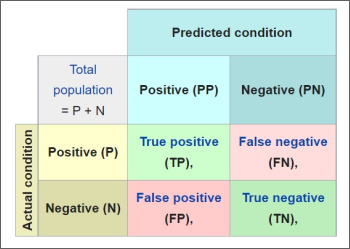
\includegraphics[scale=0.4]{2022-12-01_08_21_09.png}\\
\hline
Impact of False Positives vs False Negatives & 
Depending on the use case, the impact of false positives and false negatives are different. For example giving a healthy person a diagnosis of sick in terms of corona might leave them at home for a few days, but other than their employer, noone gets impacted. With a false negative however, they will spread the disease, creating a potential chain of events that leaves thousands of people sick. Hence, in this case, the impact of a false negative is way worse than a false positive.\\
\hline
\end{tabular}
\end{table}
\pagebreak 
\begin{table}[ht!]
\begin{tabular}{|m{0.2\linewidth}|m{0.755\linewidth}|}
\hline
Matrix Recall \textcolor{OliveGreen}{False Negatives are worse}&
This matrix \textbf{treats false negatives as worse}, this also means that it will have \textbf{more false positives}.\newline
\large \textcolor{purple}{\( \text{Recall} = \dfrac{TP}{TP + FN} \)}\newline
\normalsize \, \newline
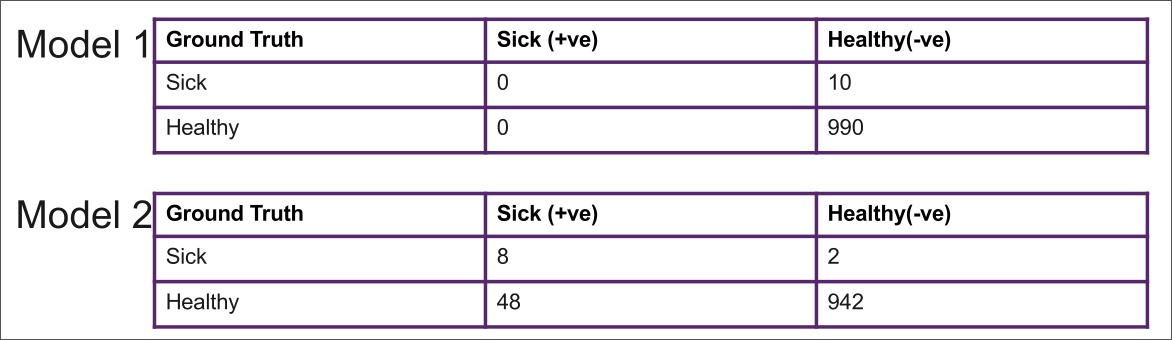
\includegraphics[scale=0.3]{2022-12-01_08_38_24.png}\newline
As one can see here, the value of Recall in model 1 is 0, we have no true positives, so 0 divided by anything is 0.\newline
And the second model has a Recall value of 0.8, so this model is better according to the recall method.\newline
\textcolor{orange}{Note that you now have values only based on false negatives and true positives, everything else is completely disregarded,\newline
you can bs this model by saying that you only have true positives, doesn't matter if you have and false positives, as they are not in the calculation.}\newline
Legend:\newline
\begin{itemize}
\item \textcolor{black}{TP = True Positives}
\item \textcolor{black}{FN = False Negative}
\item -ve (simply the negative value for this case, aka false)
\item +ve (simply the positive value for this case, aka true)\newline
  \textcolor{red}{both of these do not define if they are true positive, false positive, etc}
  \vspace{-3mm}
\end{itemize} \\
\hline
Matrix Precision \textcolor{OliveGreen}{False Positives are worse}&
This matrix \textbf{treats false positives as worse}, this also means that it will have \textbf{more false negatives}.\newline
\large \textcolor{purple}{\( \text{Recall} = \dfrac{TP}{TP + FP} \)}\newline
\normalsize \, \newline
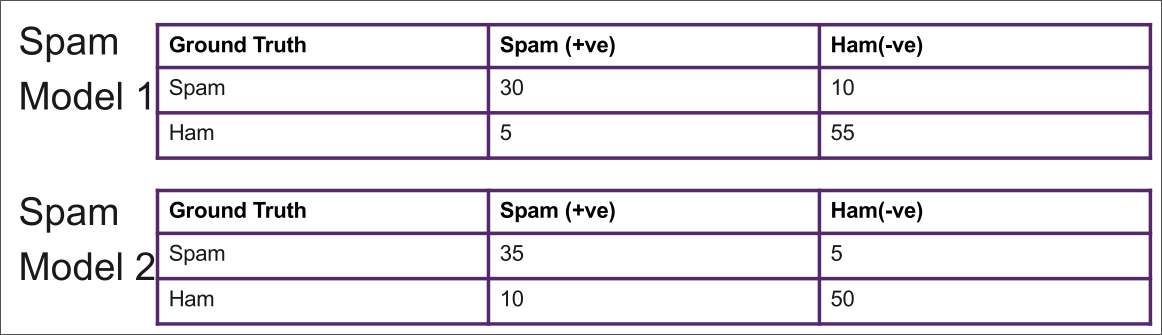
\includegraphics[scale=0.3]{2022-12-01_08_47_44.png}\newline
1. Model Precision value of 0.857\newline
2. Model Precision value of 0.777\newline
So the first model is better for Precision here.\newline
Legend:\newline
\begin{itemize}
\item \textcolor{black}{TP = True Positives}
\item \textcolor{black}{FP = False Positives}
\item -ve (simply the negative value for this case, aka false)
\item +ve (simply the positive value for this case, aka true)\newline
  \textcolor{red}{both of these do not define if they are true positive, false positive, etc}
  \vspace{-3mm}
\end{itemize}\\ 
\hline
F1 Score & 
This is the combination of both Recall and Precision.\newline
\large \textcolor{purple}{\( F1 = \dfrac{2PR}{P+R} \)}\newline
\normalsize \, \newline
If both Recall and Precision are high, then F1 is high.\newline
If one of them is low, then F1 is low.\newline
Legend: \newline
\begin{itemize}
\item \textcolor{black}{R = Recall}
\item \textcolor{black}{P = Precision}
\vspace{-3mm}
\end{itemize} \\
\hline
\(F_\beta\) & 
This is used to dial the bias to each method R, P or F1.\newline
\large \textcolor{purple}{\( F_\beta = \dfrac{(1+\beta^2)* P * R}{\beta^2 * P + R} \)}\newline
\normalsize \, \newline
Depending on the value of beta, we can dial the intensity of each method.\newline
For example, if we put beta to 0, we would get P, while if it would be 0, then we would get F1.\newline
Legend: \newline
\begin{itemize}
\item \textcolor{black}{P = Precision}
\item \textcolor{black}{R = Recall}
\item \textcolor{black}{\(F_\beta\) = bias to dial}
\item \textcolor{purple}{if \(F_\beta = 1\) then \(F_\beta \text{=>} F1 \)}
\item \textcolor{purple}{if \(F_\beta = 0\) then \(F_\beta \text{=>} P \)}
\item \textcolor{purple}{if \(F_\beta = \infty\) then \(F_\beta \text{=>} R \)}
\vspace{-3mm}
\end{itemize}\\ 
\hline
\end{tabular}
\end{table}
\pagebreak 
\begin{table}[ht!]
\begin{tabular}{|m{0.2\linewidth}|m{0.755\linewidth}|}
\hline
Receiver Operating Characterisits (ROC) &
This is a graph based on the occurrence of true and false positives.\newline
Aka how many false positives in relation to true positives.\newline
We can also look at it as an area under the curve, the bigger this area is, then the higher the ratio of true positives to false positives, and the better the quality of the model.\newline
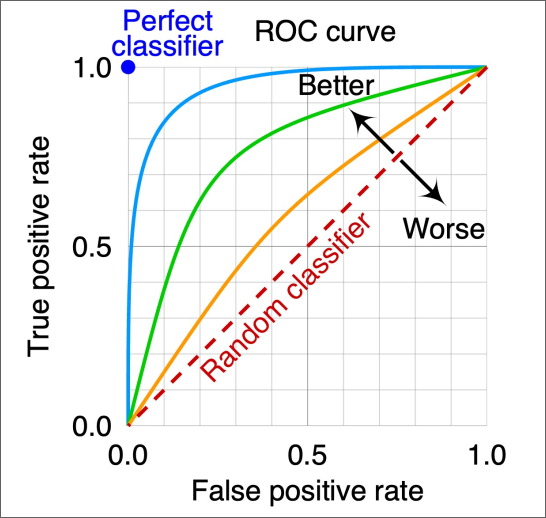
\includegraphics[scale=0.3]{2022-12-01_09_15_31.png}\\
\hline
Decision Boundary Calculation &
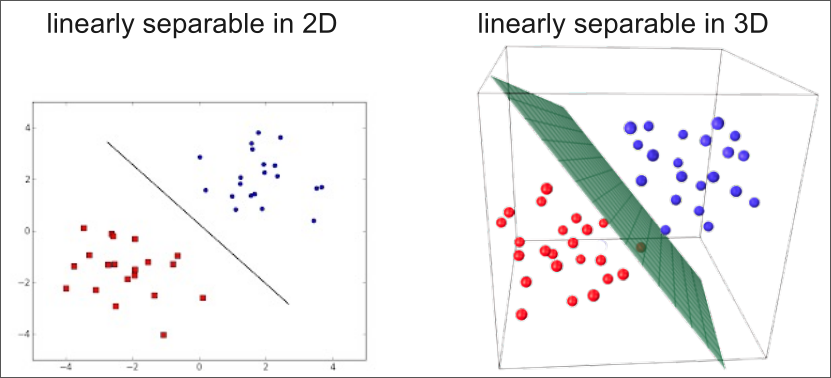
\includegraphics[scale=0.3]{2022-12-01_09_27_01.png}\newline
\large \textcolor{purple}{\(p(x) = \dfrac{1}{1 + e^{-(w_0 + w_1x_1 + w_2x_2)}}\)}\newline
\normalsize \, \newline 
Legend: \newline
\begin{itemize}
\item \textcolor{black}{p(x) = boundary}
\item \textcolor{black}{w = parameter}
\vspace{-3mm}
\end{itemize}\\ 
\hline
Polynomial Decision Boundary & 
Sometimes we have a model that we can't caluclate with a regular linear boundary, here we need something of higher order,\newline
which can draw that graph that we want.\newline
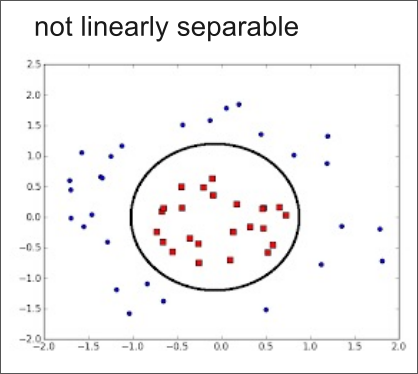
\includegraphics[scale=0.3]{2022-12-01_09_24_40.png}\newline
\large \textcolor{purple}{\(p(x) = \dfrac{1}{1 + e^{-(w_0 + w_1x_1^2 + w_2x_2^2)}}\)}\newline
\normalsize \, \newline 
Legend: \newline
\begin{itemize}
\item \textcolor{black}{p(x) = boundary}
\item \textcolor{black}{w = parameter}
\vspace{-3mm}
\end{itemize}\\ 
\hline
Multi Class classification & 
Sometimes we have multiple classes that we want to classify, for example the thousands of classes of corona...\newline
Here logistics regression has 2 methods, \textbf{One vs Rest and One vs One}.\newline
\begin{itemize}
\item \textcolor{Purple}{One vs Rest}:\newline
\begin{itemize}
\item This trains a single calssifier for each class and train data to them.
\item Fit data to each class just like we did before with singular classes.
\item \textcolor{orange}{The classifier that reports the highest probability P is the class that we get.}
\end{itemize} 
\item \textcolor{Purple}{One vs One}:\newline
  \begin{itemize}
  \item \textcolor{black}{Train classifiers to distinguish between each pair of classes (c1,c2)(c1,c3)(c2,c3)...}
  \item \textcolor{black}{apply all classifiers to an unseen sample x -> training}
  \item \textcolor{black}{Combine the results to produce final classification}
  \end{itemize} 
\vspace{-3mm}
\end{itemize}\\ 
\hline
\end{tabular}
\end{table}
\pagebreak
\begin{table}[ht!]
\begin{tabular}{|m{0.2\linewidth}|m{0.755\linewidth}|}
\hline
KNN classification & 
This is a method to define neighbours in classes. \newline
K stands for a number, which you can define to make a boundary that defines how many neighbours will be in the group:\newline
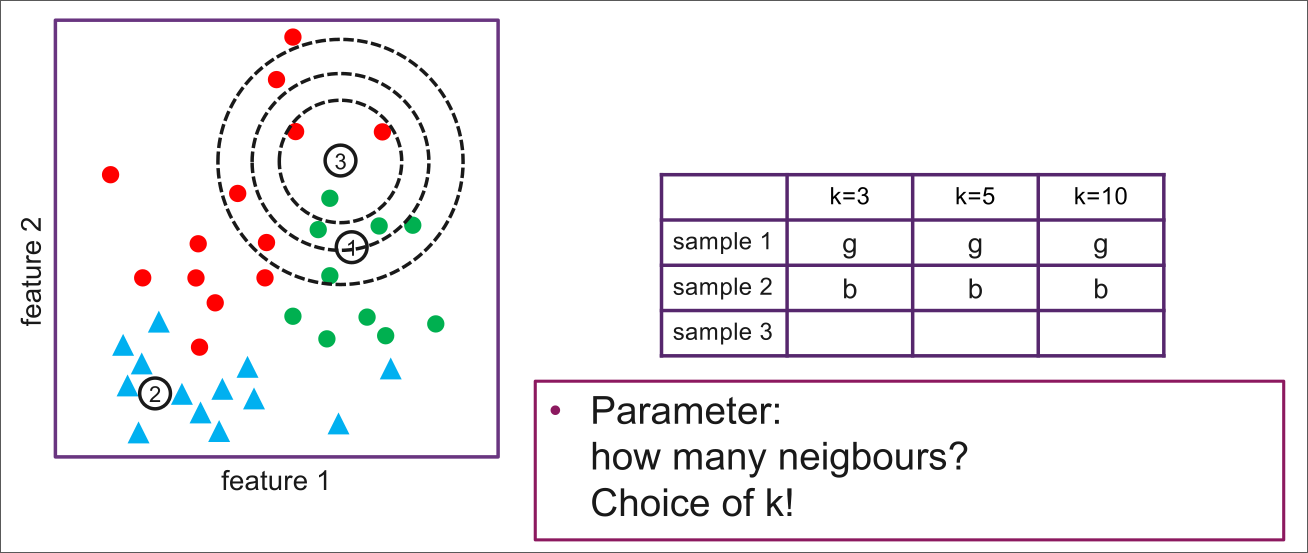
\includegraphics[scale=0.3]{2022-12-01_09_38_00.png}\newline
Then we chose a method which could be any calculation,\newline
in other words, the \textbf{near} can be: \textbf{Euclidean, Manhatten, cosine, Minkowski, or some other algorithm}.\newline
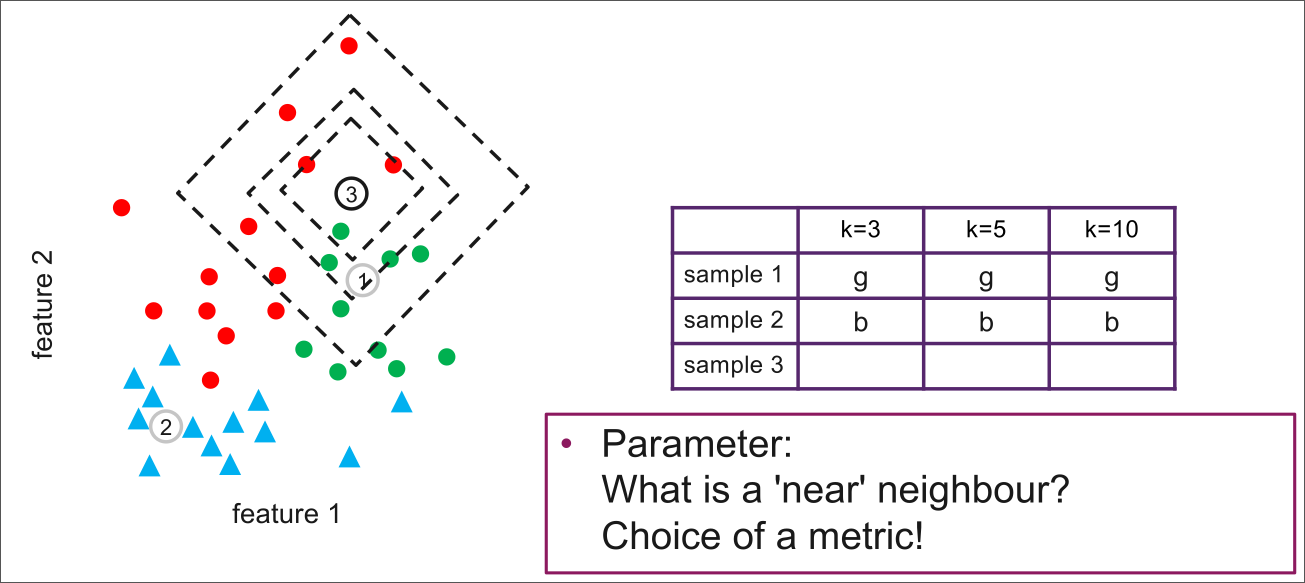
\includegraphics[scale=0.3]{2022-12-01_09_39_37.png}\newline
\textcolor{orange}{For each dataset in t-test, do the following:}\newline
\begin{itemize}
\item \textcolor{purple}{For all training data x-train, calculate the d(x-test, x-train)}
\item \textcolor{purple}{Sort training data in the ascending order of the distance}
\item \textcolor{purple}{Choose the first k data ponts from the sorted training data}
\item \textcolor{purple}{Choose the most frequent occuring class form the k data points as the classification result}
\end{itemize} 
\, \newline
Legend:\newline
\begin{itemize}
\item \textcolor{black}{d = distance metric}
\item \textcolor{black}{k = Neighbours}
\end{itemize}
\minipg{
\textcolor{OliveGreen}{Advantages:}\newline
\begin{itemize}
\item \textcolor{OliveGreen}{Easy and simple machine learning model}
\item \textcolor{OliveGreen}{Few hyperparameters needed}
  \vspace{2mm}
  \vspace{2mm}
  \vspace{2mm}
\end{itemize}
}{
\textcolor{red}{Disadvantages:}\newline
\begin{itemize}
\item \textcolor{red}{k should be wisely selected}
\item \textcolor{red}{Large computation cost during runtime if dataset is large}
\item \textcolor{red}{Not efficient for high dimensional datasets}
\item \textcolor{red}{Proper scaling should be provided for fair treatment among features}
\end{itemize} 
}[0.3,0.4]
\\ 
\hline
Distance Metric &
\vspace{2mm}
\large
\begin{itemize}
  \item \textcolor{purple}{Cosine Distance Metric: \( \theta = \dfrac{x_1 * x_2}{|x_1| * |x_2|} \)}\newline
    \, \newline
  \item \textcolor{purple}{Manhatten Distance: \( d_\text{MH}(x_1,x_2)= \sum_{i=1}^{p} | x_{i,1} - x_{i,2} | \)}\newline
    \, \newline
  \item \textcolor{purple}{Euclidean Distance: \( d_E(x_1,x_2) = \sqrt{\sum_{i=1}^{i=p}(x_{i,1} - x_{i,2})^2} \)}\newline
    \textcolor{red}{Most used}
  \item \textcolor{purple}{Minkowski Distance: \( d_{MK}(x_1,x_2) = (\sum_{i=1}^{p}(|x_{i,1} - x_{i,2}|^p))^{\dfrac{1}{p}} \)}
\vspace{-3mm}
\end{itemize} 
\normalsize \, \newline
There are special cases for manhatten at p = 1, and at eucledian for p = 2\newline
Here a small comparison: \newline
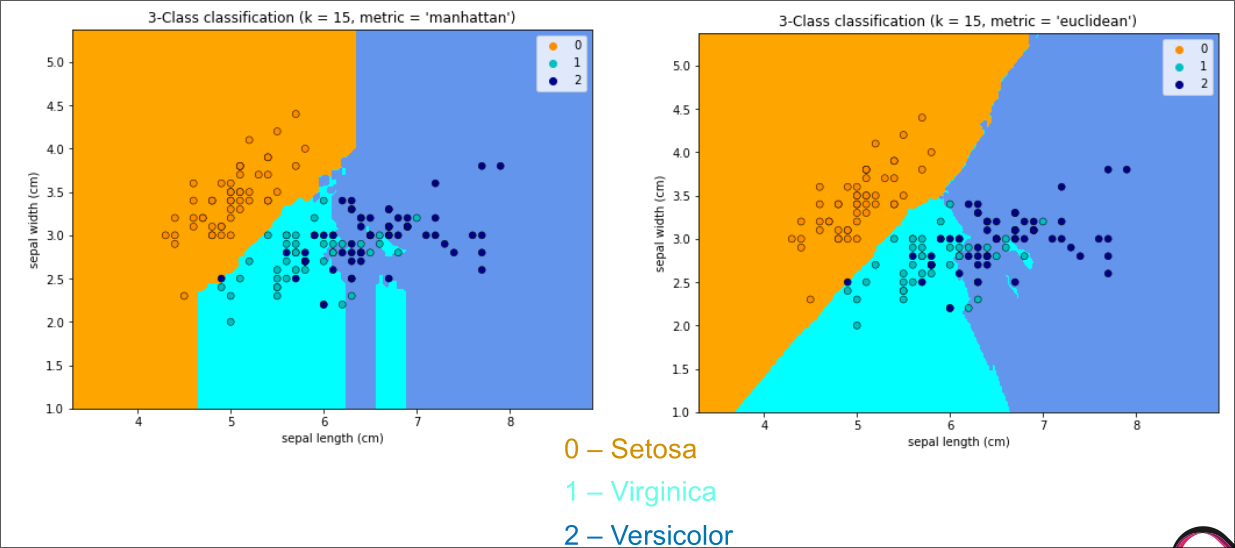
\includegraphics[scale=0.25]{2022-12-01_09_53_58.png}\\
\hline
\end{tabular}
\end{table}
\pagebreak
\begin{table}[ht!]
\begin{tabular}{|m{0.2\linewidth}|m{0.755\linewidth}|}
\hline
K and Variance/Bias & 
\textcolor{purple}{\textbf{The higher k} is, the \textbf{higher the variance} is, therefore the \textbf{model is more complex}, when you have \textbf{less k, the model gets simpler}, making you have \textbf{more bias}.\newline
Therefore, the best solution is to have a sweetspot of both complexity and bias, as already covered earlier.}
\\
\hline
Naive Bayes Classification & 
\textcolor{purple}{Calculate the posterior probability based on the previous state.}\newline
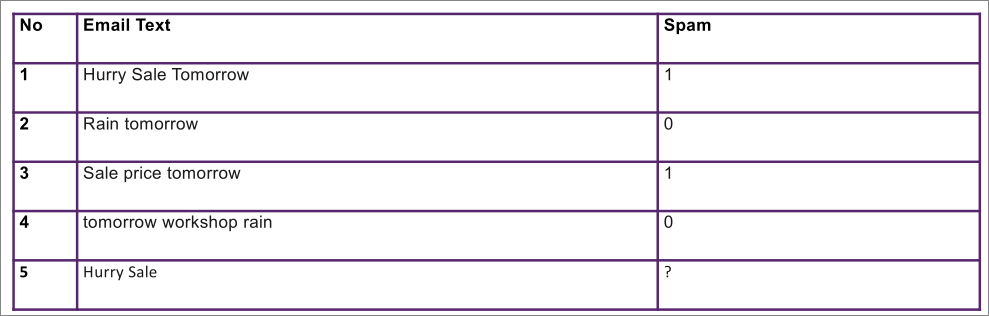
\includegraphics[scale=0.3]{2022-12-08_11_03_47.png}\newline
Remember conditional probability:\newline
\, \newline
\large \textcolor{purple}{\( Pr(e | D) = \dfrac{Pr(D,e)}{Pr(e)} \)}\newline
\normalsize \, \newline
Let's say we want to see if an email is spam based on whether or not it has a word in it, let's take hurry for this:\newline
Then we calculate it like this:\newline
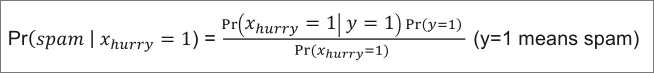
\includegraphics[scale=0.4]{2022-12-08_11_10_40.png}\newline
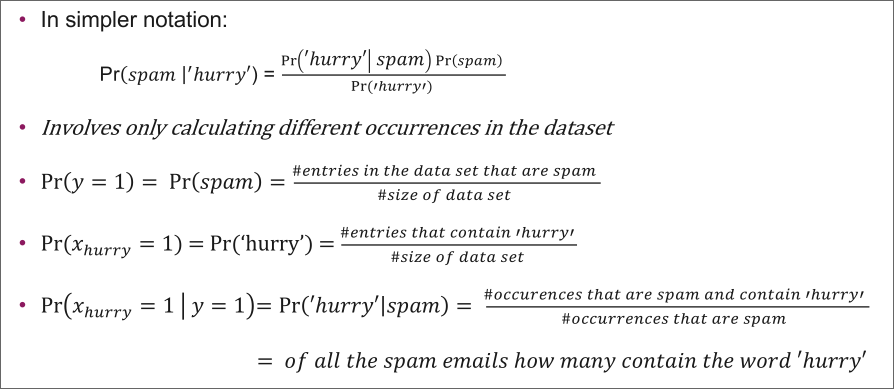
\includegraphics[scale=0.4]{2022-12-08_11_12_45.png}\newline
\begin{itemize}
\item \textcolor{OliveGreen}{good when dataset is small}
\item \textcolor{OliveGreen}{No training}
\item \textcolor{OliveGreen}{No explicit training phrase}
\item \textcolor{OliveGreen}{generative class of models}
\item \textcolor{OliveGreen}{used extensively when data contains categorical features but not much used in numerical features}\newline
You could theoretically convert numerical values into categorical values, making it feasible again with naive bayes.
\vspace{-3mm}
\end{itemize} 
\\
\hline
\end{tabular}
\section{Unsupervised Learning}
\begin{tabular}{|m{0.2\linewidth}|m{0.755\linewidth}|}
\hline
Basics & 
Unsupervised learning deals with data where we do not have labels, this means that we can't manually intervene, since we do not have any hints to do so.\newline
Remember the flower example we used for KNN, there we had 3 different labels for flowers, so we knew how to categorize, but what if we do not have the flower types? How would we categorize the data?\newline 
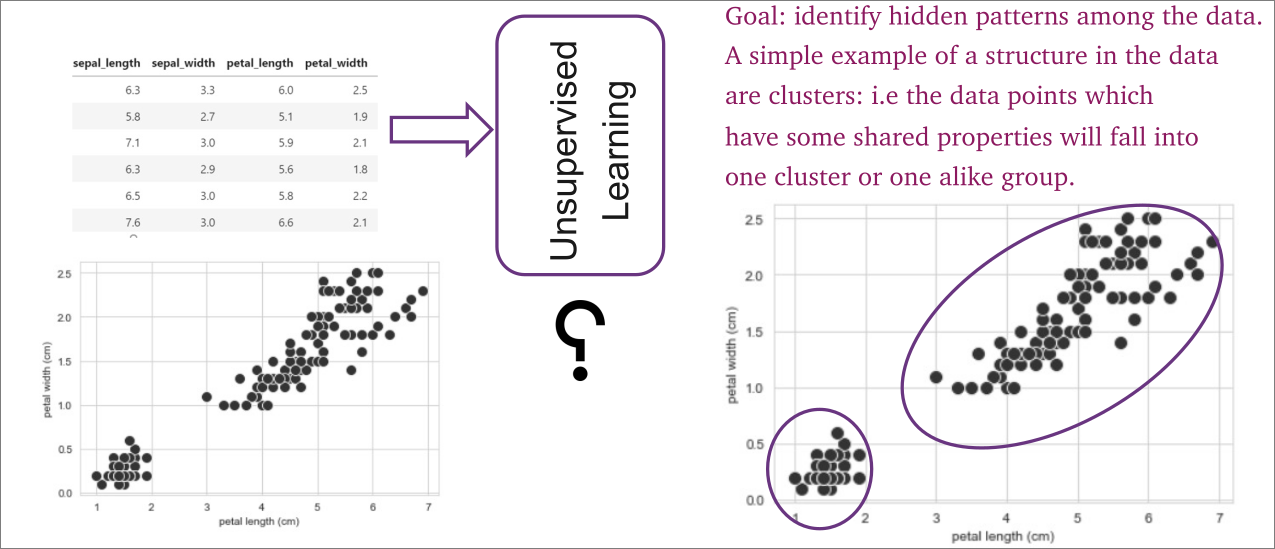
\includegraphics[scale=0.3]{2022-12-08_11_22_47.png}\newline
As you can see this is still the same example, but how do we figure out wich Y value belongs together? If we remember the flower example, we know that we have 3 groups, but here we can only clearly seperate 2 groups... The answer can be found in the next entry -> \textbf{Clustering!}
\textcolor{orange}{This is usually used in social network analysis, astronomical data, market segmentation and more.}\\
\hline
Clustering & 
The idea of clustering is the same as with KNN, we try to group data into seperate clusters.\newline
\textcolor{orange}{Group \textbf{n} datapoints into \textbf{\(k_c\)} number of clusters}\newline
\\
\hline
\end{tabular}
\end{table}
\pagebreak
\begin{table}[ht!]
\subsection{Clustering}
\begin{tabular}{|m{0.2\linewidth}|m{0.755\linewidth}|}
\hline
Steps For Clustering &
\vspace{2mm}
\begin{enumerate}
\item \textcolor{purple}{Choose the amount of clusters that you want/need: \(k_c\) cluster amount}
\item \textcolor{purple}{For each cluster (\(C_1, C_2, C_{k_c}\)), choose a random center, or calculate it }\newline
\item \textcolor{purple}{Assignment:}\newline
  \begin{enumerate}
  \item \textcolor{orange}{Find the \textbf{squared Euclidean distance} (or other method) between the centers and all the data points}\newline
    \, \newline
    \large  \textcolor{purple}{\(\sum_{i=1}^{k_c} \sum_{j=1}^{N} d_{i,j} = (x_j - C_i)^2\)}\newline
    \normalsize \, \newline
    x is a datapoint of N datapoints , and C is a center of \(k_c\) Centers.\newline
  \item \textcolor{orange}{Assign each data point to the cluster of the \textbf{nearest center -> Lowest Euclidean Distance}}
  \end{enumerate} 
\item \textcolor{purple}{Update: Each clustern now has a potential new center(mean). we do this by \textbf{calculating the new center!}}\newline
  \, \newline
  \large \textcolor{purple}{\( \text{new Center} = \text{new Center X + new Center Y}\newline
    \, \newline
  new Center = \dfrac{x_1, x_2 , \text{...}, x_{N}}{N} \dfrac{y_1, y_2 , \text{...}, y_{N}}{N} \)}\newline
  \normalsize \, \newline
\item \textcolor{purple}{If some stopping criteria is met, stop}\newline
  \begin{itemize}
  \item \textcolor{orange}{When centers don't change}
  \item \textcolor{orange}{Datapoints remain in the same clusters, even though centers change -> takes too much time}
  \item \textcolor{orange}{The distance of datapoints to their centers is greater than a threshold we set}
  \item \textcolor{orange}{Fixed number of iterations have been reached -> similar to max recursion}
  \end{itemize} 
  \textcolor{orange}{Or the center didn't change from the last step!}
\item \textcolor{purple}{Else, go to step 3}
\end{enumerate}
Example Assignment:\newline
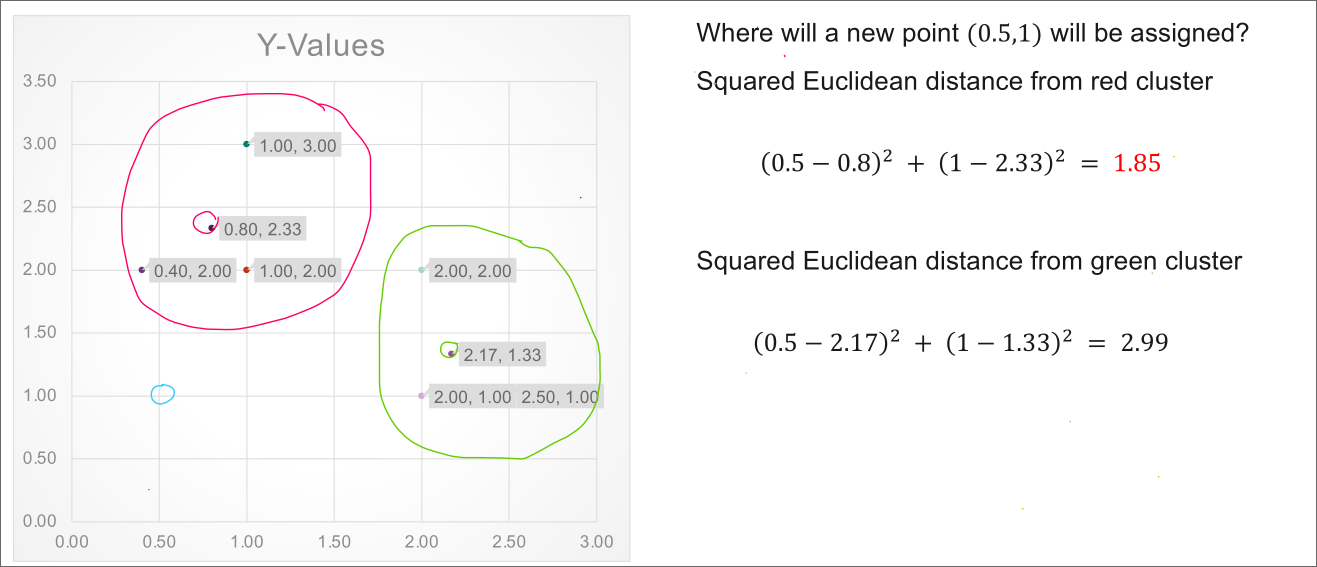
\includegraphics[scale=0.3]{2022-12-08_12_42_29.png}\newline
Example New Center Calculation:\newline
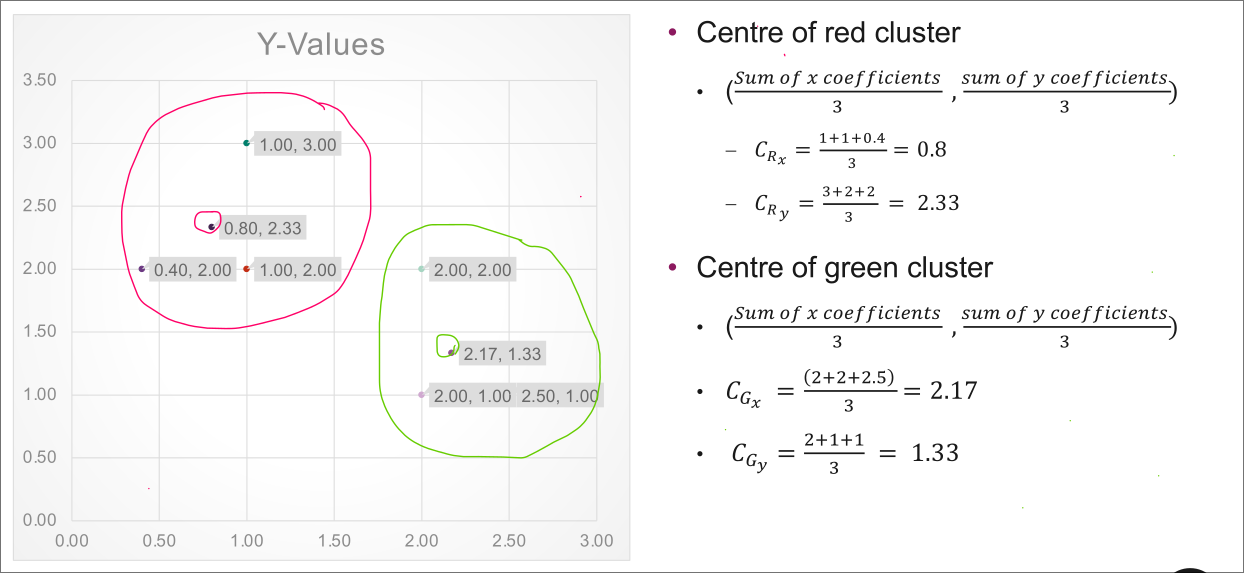
\includegraphics[scale=0.3]{2022-12-08_12_42_35.png}\newline
Notes: \newline
\begin{itemize}
\item \textcolor{purple}{Performance}\newline
\textcolor{orange}{Performance is heavily dependent on the initial random seed, if the random seed takes datapoints close together, then you will have many center changes, therefore you will have lots of computation that could be avoided.}\newline
You can solve this by either \textbf{manually chosing the initial clusters}, or you can \textbf{run the initial step multiple times, until a suitable on has been found.}
\item \textcolor{purple}{Standardization}\newline
  Just like the first time we started using graph plots, when \textbf{a variable to consider has a large range}, then it will \textbf{overshadow all other variables}, therefore,\newline
  We need to \textbf{downscale this variable} in order to make the other variables also have weight in this graph.
\item \textcolor{purple}{Sklearn has implementation of this, check documentation}
\item \textcolor{purple}{Choose \(k_c\) wisely!}\newline
  Choosing \(k_c\) as 0,1 or N is useless, the first is no cluster, so what are we even doing, the scond 1 cluster, also useless\newline
  then N is each datapoint in it's own cluster, also usless... \textbf{Therefore base it on the data that you have and what you expect!}
\vspace{-3mm}
\end{itemize} 
\\
\hline
\end{tabular}
\end{table}
\pagebreak 
\begin{table}[ht!]
\begin{tabular}{|m{0.2\linewidth}|m{0.755\linewidth}|}
\hline
Problems with Clustering & 
\textcolor{red}{Clustering is only mathematical, therefore it only calculates distance. This means that sometimes you will have clusters that mathematically are indeed correct, but if a human looks at them, they make no sense, as a certain datapoint is completely isolated with a gap between other points as shown here in this example:}\newline
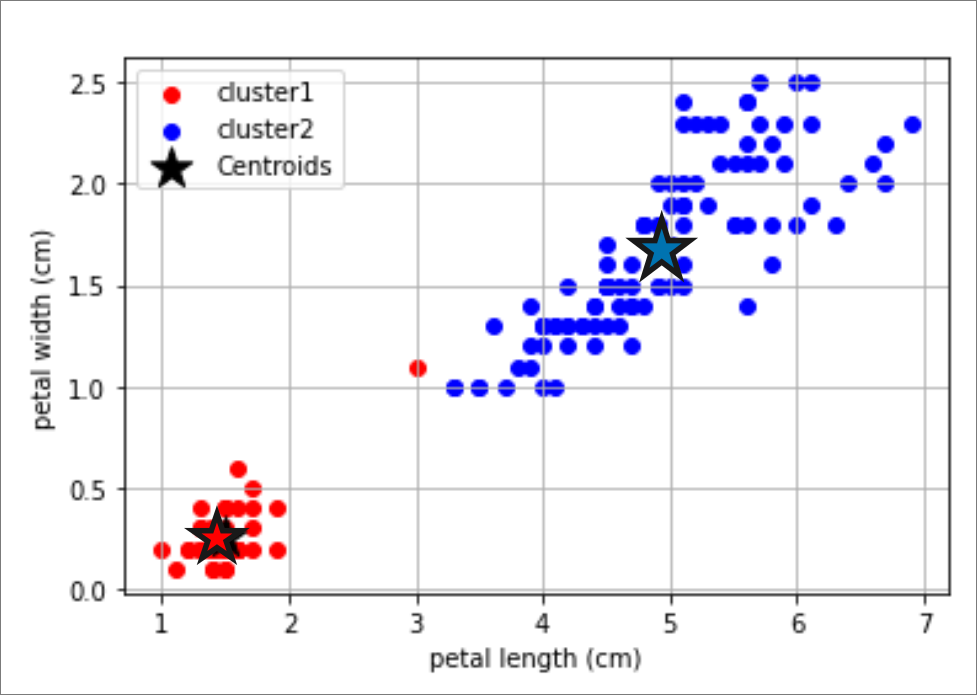
\includegraphics[scale=0.3]{2022-12-08_01_07_27.png}\newline
Here a single red dot is in the blue cluster because it is mathematically closer to the red center, but to a human this clearly doesn't make sense!!
\\
\hline
Inertia OR within-cluster sum-of-squares (WCSS) & 
This is the solution to the previous problem, here we simply \textbf{take the sum of each distance of a datapoint to the center}.\newline
\textcolor{orange}{This sum of distances should be as low as possible!}\newline
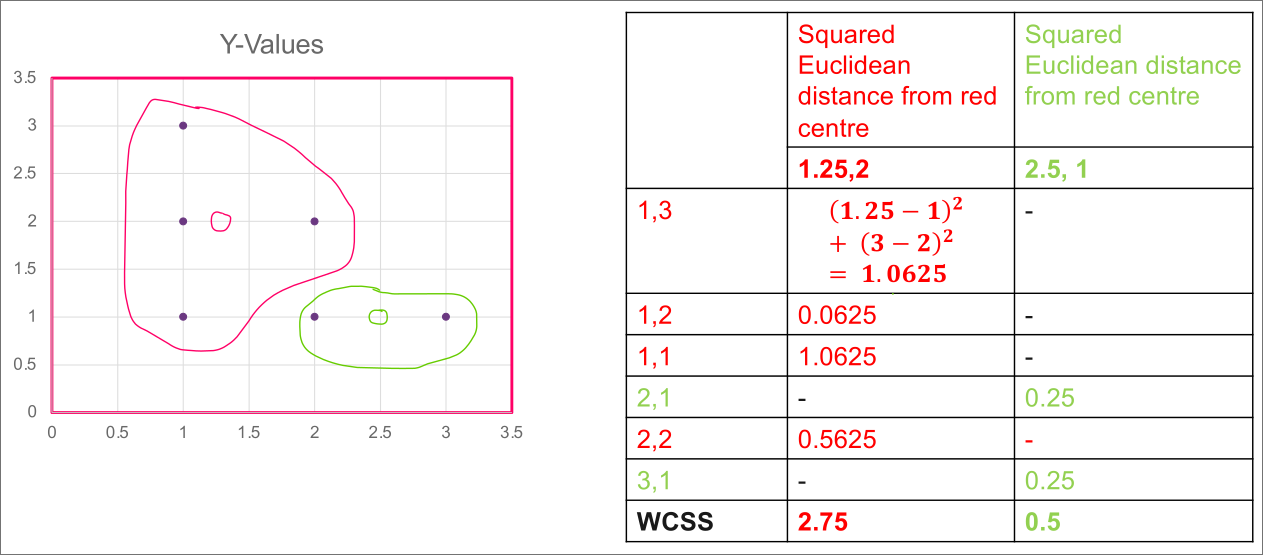
\includegraphics[scale=0.3]{2022-12-08_01_14_08.png}\newline
Here also an example with python:\newline
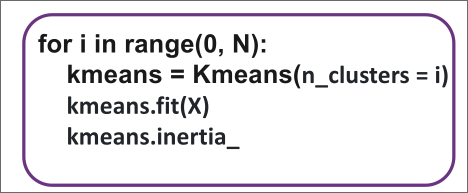
\includegraphics[scale=0.3]{2022-12-08_01_13_58.png}\newline
\textcolor{purple}{For the previous example where 1 datapoint was alone in the wrong cluster, we would get a significantly lower WCSS when we remove said problematic point, getting us a better solution!}\newline
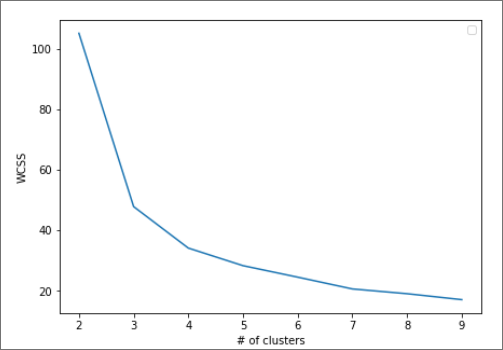
\includegraphics[scale=0.4]{2022-12-08_01_25_03.png}\newline
The more clusters you have, the smaller the WCSS gets, once again makes it clear that you want to have a \textbf{sweet spot}, between cluster count and WCSS 
\\
\hline
\end{tabular}
\end{table}
\pagebreak
\begin{table}[ht!]
\begin{tabular}{|m{0.2\linewidth}|m{0.755\linewidth}|}
\hline
Silhouette Score & 
\textcolor{orange}{This is an alternative method to WCSS and clustering, which also takes into account the coherency of clusters.}\newline
\, \newline
\large \textcolor{purple}{\( \text{Silhouette Score} = \dfrac{b - a}{max(a,b)}\)}\newline
\normalsize \, \newline
Legend: \newline
\begin{itemize}
\item \textcolor{orange}{a = intra-cluster average (average distance between each point within a cluster)}
\item \textcolor{orange}{b = inter-cluster average (average distance from a cluster to its nearest neighbour cluster)}
\item \textcolor{orange}{Range of the silhouette score is from -1 to 1 and the value should be closer to 1 than -1!}
\end{itemize} 
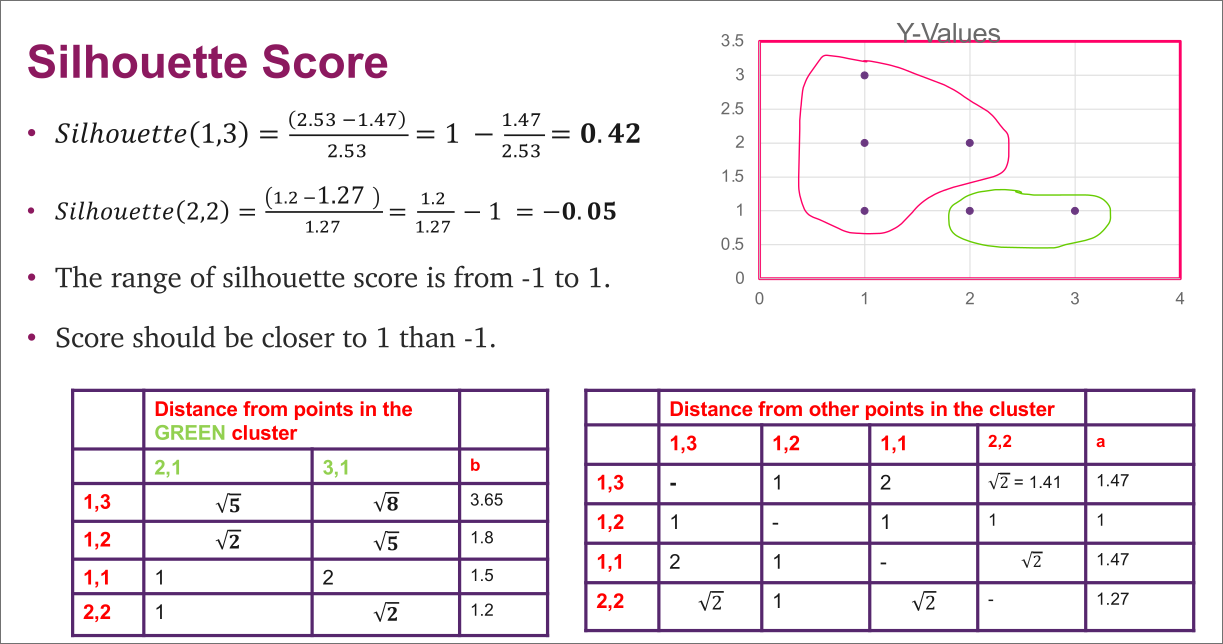
\includegraphics[scale=0.3]{2022-12-08_01_21_30.png}\newline
The mean of a and b are not shown in the tables but can be calculated as any mean can -> sum over amount of datapoints\newline
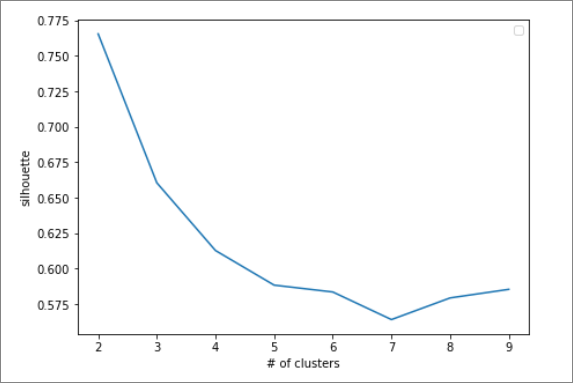
\includegraphics[scale=0.4]{2022-12-08_01_32_23.png}\newline
\textcolor{orange}{Here the lower amount of clusters the better, since the silhouette score needs to be closer to 1 than -1!}\newline
This is in contrast to WCSS where more would be better!
\\
\hline
\end{tabular}
\section{Ensemble Learning}
\begin{tabular}{|m{0.2\linewidth}|m{0.755\linewidth}|}
\hline
Wisdom of Crowds & 
The idea with ensemble learning is to try to use as many models as possible and then aggregate the results, this can often lead to an answer that is just as good as one from an expert, or here the best model.\newline
The benefit of course is that you do not have to spend any time to choose models as you simply choose all of them, with very likely an answer that will work as well!\newline
\textcolor{purple}{In certain cases, the ensemble method will provide even better results as the "specialized model for this problem."}\\
\hline
When Ensemble is strong & 
\vspace{2mm}
\begin{itemize}
\item \textcolor{purple}{Sufficient number of "weak learners" -> refers to simple models in ensemble learning}
\item \textcolor{purple}{Models make different types of errors}\newline
  Ensemble can't clean errors if the every model has the same error
\item \textcolor{purple}{Models are not trained on the same data}\newline
  Otherwise you risk getting the same error with different models
\item \textcolor{purple}{Models used are better than choosing random values}
\vspace{-3mm}
\end{itemize} 
\\
\hline
How to choose models & 
\begin{itemize}
\item \textcolor{purple}{Different Algorithms}\newline
  \begin{itemize}
  \item \textcolor{black}{KNN}
  \item \textcolor{black}{Logistic Regression}
  \end{itemize}  
\item \textcolor{purple}{Different Hyperparameters}\newline
  \begin{itemize}
  \item \textcolor{black}{KNN with various k parameters}
  \item \textcolor{black}{Regressin with regularization parameters}
  \end{itemize}  
\item \textcolor{purple}{Different training data}\newline
\vspace{-3mm}
\end{itemize} 
\\
\hline
Ways of Ensemble & 
\begin{itemize}
\item \textcolor{OliveGreen}{Voting}\newline
  \begin{itemize}
  \item \textcolor{black}{Hard Voting}
  \item \textcolor{black}{Hard Voting with Weights}
  \item \textcolor{black}{Soft Voting}
  \item \textcolor{black}{Soft Voting with Weigths}
  \end{itemize} 
\item \textcolor{OliveGreen}{Bagging(pasting)}\newline
  Train classifiers on different data
\item \textcolor{OliveGreen}{Boosting}\newline
  Train models such that model n improves on the accuracy of model n-1 -> last model
\item \textcolor{OliveGreen}{Stacking}
\item \textcolor{OliveGreen}{Blending}
\vspace{-3mm}
\end{itemize} 
\\
\hline
\end{tabular}
\end{table}
\pagebreak
\begin{table}[ht!]
\section{}
\begin{tabular}{|m{0.2\linewidth}|m{0.755\linewidth}|}
\hline
Hard Voting & 
\textcolor{red}{Majority decides}\newline
3 out of 4 models predict that the y value will be true, therefore the ensemble will also predict y as true for this data.
\\
\hline
Hard Voting with Weights & 
With weights, we can say that one model is preferred over another, therefore we can give it a bigger weight, essentially meaning that they have more votes, or more say in the vote.\newline
We do this with a set of parameters, one parameter for every model.\newline
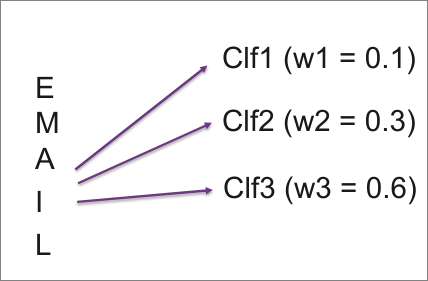
\includegraphics[scale=0.3]{2022-12-15_11_07_38.png}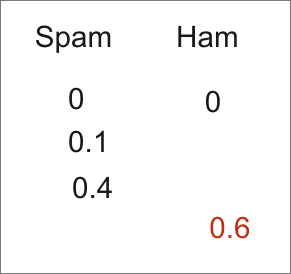
\includegraphics[scale=0.3]{2022-12-15_11_07_44.png}\newline
As you can see 2 out of 3 models said y will be spam, but the third model has more weight than both of those combined, meaning that the data will be predicted as Ham.\\
\hline
Soft Voting & 
\textbf{Here we take all predictions for value y in one model}, not just the final one.\newline
In other words, a model might predict y to be 80\% spam and 20\% ham, therefore in a regular hard vote, you would simply say the model considers y as spam, but here we take both values and add them to each respective value of the other models.\newline
At the end you take the \textbf{average of every possible prediction}, here only spam and ham, and the highest value at the end is our prediction.\newline
Here an example: \newline
\includegraphics[scale=0.3]{2022-12-15_11_10_24.png} \newline
\textcolor{red}{Important, due to the percentage being necessary, \textbf{this only works with probability}, otherwise we can't take the average of all probabilities!!}\\
\hline
Soft Voting with Weights & 
\textcolor{purple}{This is the same as soft voting, just here again, we apply a weight to each percentage of each model.}
\\
\hline
Voting Regressor & 
You can also use different regression models and combine them, this essentially just applies the regression on the entire dataset and takes the average of each regressor.
\\
\hline
Bagging Methods & 
This splits the data into random sets of data, which can be used to train all the different models that we have to train.\newline
\includegraphics[scale=0.4]{2022-12-15_11_28_43.png}\\
\hline
Sampling with Replacement & 
This treats each datapoint as a singular point, of which we essentially have a pool of. From this pool, each model takes an amount of datapoints, and \textbf{we can decide whether or not to remove points chosen from the pool and only use it on this one model, or to reuse points, essentially cloning and leaving the real one inside the pool for the next model to potentially choose.}\newline
\includegraphics[scale=0.4]{2022-12-15_11_39_41.png} \, \newline
\textcolor{red}{Sampling with replacement is also called \textbf{Bagging, or Bootstrap Aggregating}}\newline
\textcolor{red}{Sampling without replacement is also called \textbf{Pasting}} \newline 
Note, Bagging works best with strong and complex models as it can \textbf{reduce overfitting} if that is the case!\\
\hline

\hline
\end{tabular}
\end{table}
\pagebreak
\begin{table}[ht!]
\begin{tabular}{|m{0.2\linewidth}|m{0.755\linewidth}|}
\hline
Bagging Classifier & 
There are different ways of choosing data, we have learned 2 by now, but you can also combine these, meaning that you choose either bagging or pasting based on features of datasets, meaning that feature 1 will be based on bagging while feature 2 will be based on pasting. \newline
\textcolor{orange}{This would be called \textbf{Random Subspaces}}\newline
Or you can choose both features and other random subsets of data to choose either bagging or pasting from.\newline
\textcolor{orange}{This would be called \textbf{Random Patches}}
\\
\hline
Bagging Classifiers/Regressor & 
After the models are fitted, use \textbf{majority vote for classiciation tasks}, and \textbf{take the average for regresssion tasks}.\\
\hline
Out of Bag (oob) Evaluation & 
Since we only use a small subset of data on each model, we can \textbf{use the rest of the data as testing data for this model}, as that data is considered as "unknown" to that model.\newline
This makes it easy for us to validate each model, so that we do not need to further split data specifically for this usecase.\\
\hline
No free lunch theorem & 
\textcolor{purple}{This philosophy simply states that there is \textbf{no best way to do things, eg. there is no single best algorithm.}}\\
\hline
Boosting & 
This \textbf{does not split the data} like Bagging, instead it trains the models \textbf{sequentially} using a specified amount of samples -> sample = point. \newline
This means that each model will try to improve on the mistakes that the last model made, therefore the combined training error reduces.\newline
I can already see a problem with overfitting with this method. Therefore, \textbf{use weaker/simpler models when boosting!}\newline
Here an example of Boosting: \newline
\includegraphics[scale=0.3]{2022-12-15_12_10_37.png}\newline
The big points are the samples on which the model didn't do well on, this means that for the next model, \textbf{the weight on these samples is incresed}, making sure, that the next model will likely change these samples.\newline
Popular Boosting methods: \newline
\begin{itemize}
  \item \textcolor{purple}{\textbf{AdaBoost (Adaptive Boost)}}
\item \textcolor{purple}{Gradient Boosting}
\item \textcolor{purple}{Extreme Gradient Boosting}
\item \textcolor{purple}{CatBoost} 
\item \textcolor{purple}{LightGBM}
\vspace{-3mm}
\end{itemize} 
\\
\hline
AdaBoost &
\vspace{2mm}
\begin{enumerate}
\item \textcolor{purple}{assigns equal weights to each training sample (\textbf{instance weights})}
\item \textcolor{purple}{trains a model to fit the given data}
\item \textcolor{purple}{\textbf{increases the weight on the misclassified samples (instance weights)}}\newline
  These are the points that will be weighted higher for the next model, so that the next model hopefully fixes these samples.\newline
\item \textcolor{purple}{Stop if the desired number of estimators are trained}
\item \textcolor{purple}{then trains a next classifier -> step 2}
\item \textcolor{purple}{For the ensemble, each classifier's weight is calculated based on its accurary. \textbf{(predictor weight)}}\newline
  \vspace{-3mm}
\end{enumerate} 
\\
\hline
\end{tabular}
\end{table}
\pagebreak
\begin{table}[ht!]
\begin{tabular}{|m{0.2\linewidth}|m{0.755\linewidth}|}
\hline
Example for step3 & 
\vspace{2mm}
\includegraphics[scale=0.3]{2022-12-15_12_20_01.png}\newline
\includegraphics[scale=0.3]{2022-12-15_12_20_10.png}\newline
As you can see you always divide the correct points over the incorrect ones and take that value to multiply the weight of each incorrect point.
\\
\hline
Example for step 6& 
For AdaBoost this is done with \textbf{log odds ratio}, making sure that we have 0 to 1 accuracy\newline
\includegraphics[scale=0.3]{2022-12-15_12_27_56.png}
\\
\hline
Adaboost in summorization &
\vspace{2mm}
\begin{itemize}
\item \textcolor{purple}{Adaboost computes the predictions of the weak predictors}
\item \textcolor{purple}{Weights the predictions using the scores of each model}
\item \textcolor{purple}{Predicted class is the one that receives the most votes -> \textbf{Hard Voting}}
\vspace{-3mm}
\end{itemize} 
\\
\hline
\end{tabular}
\section{Deep Neural Networks}
\begin{tabular}{|m{0.2\linewidth}|m{0.755\linewidth}|}
\hline
How we found the structure of our own brain & 
\textbf{Camillo Golgi} found a way to essentially paint the neural structure of the brain. This allowed was the first time we saw the structure of the brain. 
This is the foundation of deep learning as we mimmick the neurons in the brain, and perhaps because of this discover, we might be able to properly understand the brain at some point in the future.
\\
\hline
Neuron & 
A neuron is composed of \textbf{a nucleus (the center of the neuron), dendrites (the branches away from the nucleus), and an axon (the very long extension)}\newline
\includegraphics[scale=0.3]{2022-12-22_03_00_13.png}\newline
\begin{itemize}
\item \textcolor{purple}{The dendrites interact with other neurons, meaning that they receive impulses from them}
\item \textcolor{purple}{The cell body (called Soma) generates a spike if the collective input in the dendrites passes a threshold}
\item \textcolor{purple}{The generated pulse by the cell body will then travel from the axon to other neurons. Meaning the axon is the output node while the dendrites are the input nodes.}
\item \textcolor{orange}{Connections from axons to dendrites are called \textbf{synapses}}
\end{itemize}
\, \newline
\textcolor{OliveGreen}{While one neuron might not be special, the vast amount that exist in a brain make the difference, meaning that the actual power comes from the \textbf{network}, not from the single neuron.}
\\
\hline
\end{tabular}
\end{table}
\pagebreak
\begin{table}[ht!]
\subsection{Artificial Neural Network}
\begin{tabular}{|m{0.2\linewidth}|m{0.755\linewidth}|}
\hline
Artificial Neurons &
\vspace{2mm}
\begin{itemize}
  \item \textcolor{purple}{The artificial neuron receives an input vector[x1,x2,...]}
  \item \textcolor{purple}{Each neuron has its own input weights [w1,w2,...] and \textbf{bias b} (intercept)}
\item \textcolor{purple}{The neuron calculates the sum of the weighted input (dot product x * w), adds a bias b, and passes it through a nonlinear \textbf{activation function}}
\end{itemize}
\includegraphics[scale=0.4]{2022-12-22_03_11_00.png}\newline
As you can see here, the function looks very similar to the \textbf{sigmoid} function used in logistic regression\newline 
\textcolor{red}{If you compare this to logistic regression or some other simpler form of training, then you see that we essentially do the same, just with a new model, and the only thing missing here is the loss function, which you can then choose and apply to your appropriate training/testing data!}\\
\hline
TLU (Threshold Linear Unit) & 
This is one of the simplest forms of a neuron. Here we simply put together the weights and biases with our inputs -> cross product, apply biases and then use a binary function to determine the output -> 0 or 1. \newline
\textcolor{purple}{\( \text{input} > 0 \text{ => } \text{output} == 1 \)}\newline
\textcolor{purple}{\( \text{input} \leq 0 \text{ => } \text{output} == 0 \)}\newline
\includegraphics[scale=0.4]{2022-12-22_03_18_57.png}
\\
\hline
Perceptron & 
A single layer of TLUs (multople TLU in a row) is called perceptron, here the following things must be guaranteed in order for the TLU to be a perceptron:\newline
\begin{itemize}
\item \textcolor{purple}{Each TLU must be connected to all inputs}
\item \textcolor{purple}{Bias node is 1, however, the actual bias will then transform this, hence bias = 1 * b1!!!}
\item \textcolor{purple}{Each TLU might have different weights, which make the difference}
\item \textcolor{purple}{Mutli class classification is easily possible}
\item \textcolor{purple}{Linear decision boundary due to 0 and 1 constraint}
\item \textcolor{purple}{Can't learn complex patterns}
\item \textcolor{purple}{Included in Sklearn}
\end{itemize} 
\, \newline
\includegraphics[scale=0.4]{2022-12-22_03_29_14.png}
\\
\hline
AND gate with Perceptron & 
We can crate AND with weights and 2 inputs, consider the caption below with the following inputs from the table:\newline
\begin{itemize}
\item \textcolor{black}{x1=0, x2=0, output = (20 * 0 + 20 * 0) -30 (bias) => -30}
\item \textcolor{black}{x1=1, x2=0, output = (20 * 1 + 20 * 0) -30 (bias) => -10}
\item \textcolor{black}{x1=0, x2=1, output = (20 * 0 + 20 * 1) -30 (bias) => -10}
\item \textcolor{black}{x1=1, x2=1, output = (20 * 1 + 20 * 1) -30 (bias) => 10}
\end{itemize} 
\includegraphics[scale=0.4]{2022-12-22_03_38_24.png}
\\
\hline
\end{tabular}
\end{table}
\pagebreak
\begin{table}[ht!]
\begin{tabular}{|m{0.2\linewidth}|m{0.755\linewidth}|}
\hline
OR gate with Perceptron & 
\vspace{2mm}
\begin{itemize}
\item \textcolor{black}{x1=0, x2=0, output = (40 * 0 + 40 * 0) -30 (bias) => -30}
\item \textcolor{black}{x1=1, x2=0, output = (40 * 1 + 40 * 0) -30 (bias) => 10}
\item \textcolor{black}{x1=0, x2=1, output = (40 * 0 + 40 * 1) -30 (bias) => 10}
\item \textcolor{black}{x1=1, x2=1, output = (40 * 1 + 40 * 1) -30 (bias) => 50}
  \vspace{-3mm}
\end{itemize} 
\, \newline
As you can see, you just needed to change the weights of the data!
\\
\hline
Multi Layer Perceptron (MLP :) ) & 
\textcolor{purple}{A regular Perceptron can't create things such as \textbf{XOR}, when we use multiple layers we can remove some of these constraints.}\newline
This is also called \textbf{Artificial Neural Network (ANN).}\newline
As you can see below, each next layer treats the previous neurons as inputs, this means that you can increase the complexity of the neural network depending on the amount of layers \textbf{(depth)} and with the amount of neurons that you place in a layer.\newline
At the end it also matters how complex your \textbf{activation function in each neuron is!}\newline
\includegraphics[scale=0.4]{2022-12-22_03_54_40.png}\\
\hline
Training a neural network & 
When trying to train a neural network, we need to represent the training in the weights, just like with gradient descent.\newline
\includegraphics[scale=0.4]{2022-12-22_04_14_24.png}\newline
As one can see, the we calculate the loss and apply it to the weight, problem is, we need to propagate this wo each other neuron that also has this input, how can we do this?\newline
There are a few ways to do it:\newline
\begin{itemize}
\item \textcolor{purple}{Partial derivatives -> Pen and paper, very tedious, not automated}
\item \textcolor{purple}{Numeric Differentiation, imprecise, approximated}\newline
\includegraphics[scale=0.4]{2022-12-22_04_18_04.png}
\item \textcolor{purple}{Symbolic Differentiation}\newline
  \begin{itemize}
  \item \textcolor{black}{For complicated functions, the resultant expression can be exponentially large}
  \item \textcolor{black}{Touch to simplify and leads to suboptimal performance}
  \item \textcolor{black}{Wasteful to keep around intermediate symbolic expressions if we only need a numeric value of the gradient in the end}
  \item \textcolor{black}{Prone to error}
  \end{itemize} 
\item \textcolor{purple}{Reverse-mode autodiff}
\vspace{-3mm}
\end{itemize} 
\\
\hline
Reverse-mode autodiff  & 
This essentially does the same as with pen and paper, just that we use \textbf{Backwards Propagation}\newline
\includegraphics[scale=0.4]{2022-12-22_04_22_59.png}
\\
\hline
\end{tabular}
\end{table}
\pagebreak
\begin{table}[ht!]
\begin{tabular}{|m{0.2\linewidth}|m{0.755\linewidth}|}
\hline
&
\vspace{2mm}
\includegraphics[scale=0.4]{2022-12-22_04_27_27.png}\\
\hline
Soft max function & 
This essentially summarizes the probability of the output being of a certain class, aka the picture belonging to the class of human or of pony.\newline
\includegraphics[scale=0.4]{2022-12-22_04_24_51.png}
\\
\hline
\end{tabular}
\end{table}
\end{document}
